 
%%%%%%%%%%%%%%%%%%%%%%%%%%%%%%%%%%%%%%%%%%%%%%%%%%%%%%%%%%%%
%%%%%%%%%%%%%%%%%%%%%%%%%%%%%%%%%%%%%%%%%%%%%%%%%%%%%%%%%%%%
%%%%%%%%%%% Modelo-Proyecto-Monografía-Artículo %%%%%%%%%%%%
%%%%%%%%%%%%%%%%%%%%%%%%%%%%%%%%%%%%%%%%%%%%%%%%%%%%%%%%%%%%
%%%%%%%%%%%%%%%%%%%%%%%%%%%%%%%%%%%%%%%%%%%%%%%%%%%%%%%%%%%%

\documentclass[letterpaper,spanish,reprint,nofootinbib,showkeys,aps]{revtex4-2}
%\documentclass[letterpaper,spanish,preprint,,,aps]{revtex4-2}
\usepackage[paperwidth=210mm,paperheight=297mm,centering,hmargin=1.7cm,vmargin=1.7cm]{geometry}
%%%paquetes usuales%%%
\usepackage[utf8]{inputenc}%codificación
\usepackage{csquotes}
\usepackage[spanish, mexico
]{babel}%Paquete de caracteres y títulos en español de méxico

\usepackage{floatrow}

\usepackage{verbatim}%comentarios en bloque
%\usepackage{circuitikz}
\usepackage{amsmath, mathtools}%Paquete para insertar símbolos matemáticos
\usepackage{amsbsy}
\usepackage[bitstream-charter]{mathdesign}
\usepackage[mathcal]{eucal}
\DeclareSymbolFont{usualmathcal}{OMS}{cmsy}{m}{n}
\DeclareSymbolFontAlphabet{\mathcal}{usualmathcal}

\usepackage{textcomp}
\usepackage{textcomp,gensymb}
\usepackage{enumitem}
\usepackage[dvipsnames,table,xcdraw, rgb]{xcolor}
%%%Mejora la distribución de espacios%%%
\usepackage{microtype}
\usepackage[font=scriptsize,labelfont=bf]{caption}
\addto\captionsspanish{\renewcommand{\figurename}{Fig.}}

\usepackage[labelformat=simple]{subcaption}
\renewcommand*{\thesubfigure}{\alph{subfigure})}

%%%Fasores%%%
\usepackage{steinmetz}

%%%Figuras%%%
\usepackage{graphicx}
\usepackage{float}
%\usepackage{tikz,pgfplots}
%\pgfplotsset{compat=newest}

\usepackage{physics} %Un gran paquete que facilita el uso de muchas notaciones en física, y que reemplaza otras cosas por una opción más bonita, diría yo
\usepackage{bigints} %Puede hacer símbolos de integral más grandes

\usepackage{nicefrac,xfrac}

\usepackage{bm}
\usepackage{changepage} % for adjusting margins

\usepackage{listings}
\usepackage{adjustbox}
\usepackage{datetime}
\usepackage{resizegather}
%%%Definiendo colores%%%

\usepackage{lmodern}

\definecolor{dkgreen}{rgb}{0.0,0.6,0.0} 
%\definecolor{blue}{rgb}{1.0,0.49,0.0}

%%%Algunos comandos útiles para el PDF generado%%%
\usepackage[unicode=true,pdfusetitle,
 bookmarks=true,bookmarksnumbered=false,bookmarksopen=false,
 breaklinks=false,pdfborder={0 0 1},backref=false,colorlinks=true]
 {hyperref}
\hypersetup{
 citecolor=dkgreen,linkcolor=blue,urlcolor=blue}

\graphicspath{{img/}} %Setting the graphicspath


\makeatletter
\def\@fnsymbol
#1{\ensuremath{\ifcase#1\or *\or \dagger\or \ddagger\or
   \mathsection\or \mathparagraph\or \|\or **\or \dagger\dagger
   \or \ddagger\ddagger \else\@ctrerr\fi}}
\makeatother

\DeclareCaptionType{eqtag}[][Lista de ecuación.]
\captionsetup[eqtag]{labelsep=period, name=Ecuación, skip=0.15\baselineskip}

\renewcommand{\thefootnote}{\fnsymbol{footnote}}

\newcommand{\cita}[1]{\textsuperscript{\textbf{\cite{#1}}}} % este es para que la cita se vea en superíndice para ieee, si usan otro formato bórrenlo
 \newcommand{\ut}[1]{\textbf{#1}} %les hace escribir menos si quieren poner negritas en texto y mate
 \newcommand{\um}[1]{\boldsymbol{#1}}
 \renewcommand{\thefootnote}{\Roman{footnote}} %los pie de pagina los pone en letras romanas
 \newcommand{\dbar}{\text{\dj}}
 \newcommand{\parentesis}[1]{\left(#1\right)}
 \newcommand{\crch}[1]{\left[#1\right]}
\newcommand{\fn}[1]{\mathrm{#1}}
\newcommand{\fno}[1]{\mathrm{#1}(\omega)}
\newcommand{\fnv}[2]{\mathrm{#1}(#2)}

\lstset{
    inputencoding=utf8,
    extendedchars=true,
    literate={á}{{\'a}}1 {é}{{\'e}}1 {í}{{\'i}}1 {ó}{{\'o}}1 {ú}{{\'u}}1
            {Á}{{\'A}}1 {É}{{\'E}}1 {Í}{{\'I}}1 {Ó}{{\'O}}1 {Ú}{{\'U}}1
            {ñ}{{\~n}}1 {Ñ}{{\~N}}1
}

\begin{document}

\allowdisplaybreaks

\title{Determinación del gas contenido en un tiratrón 2D21, mediante la obtención de la primer energía de ionización.}

\author{ Pérez Flores Julio Alfonso}
\email{julio_perez@ciencias.unam.mx}

\affiliation{Facultad de Ciencias, Universidad Nacional Autónoma de México.}
\thanks{Reporte práctica Laboratorio Contemporánea II, Semestre 2025-1.}

%\newdate{date}{17}{06}{2024}
\date{\today}


\begin{abstract}

Se determinó un valor promedio de la primer energía de ionización del gas dentro de un tiratrón 2D21, obteniendo un valor de \ut{10.59 eV}, con un intervalo de confianza de \ut{0.8 eV}, medición la cual se aproxima con un error porcentual del \ut{1.54 \%} al valor de ionización del vapor de mercurio, gas utilizado en el diseño de este tiratrón. Estos valores se  obtenieron mediante el análisis de las curvas de corriente en función de $V^{\nicefrac{3}{2}}$, así como ajustes por mínimos cuadrados de la región lineal, suavización de curvas utilizando el método LOESS y derivación numérica. Se pudieron identificaron las tres regiones clave: la región gobernada por la ley de Child-Langmuir, la zona de transición y la zona de saturación. Este método, además de validar la presencia de mercurio en el bulbo del tiratrón, destaca por su precisión y ofrece un enfoque reproducible para estudios similares. Así mismo se realizó una discusión sobre mejoras instrumentales para reducir el ruido experimental y optimizar futuros análisis. 
 
\end{abstract}


\keywords{2D21 Tyratron, first ionizing energy, Child-Langmuir law.}

\maketitle


\section{ Introducción}\label{sec:introduccion}


El potencial de ionización es la energía mínima necesaria para arrancar un electrón de un átomo o ion en su estado gaseoso y en su nivel más externo corresponde a un electron en la capa de valencia, esta energía  indica la probabilidad de que un átomo forme un catión y, de ser así, qué carga tendría. En términos generales, refleja qué tan fuertemente está unido un electrón al núcleo y cuán estable es. Además, permite inferir las energías de los orbitales reales, los efectos que los electrones ejercen entre sí, y ayuda a predecir la reactividad química y las propiedades de las moléculas \cite{emily}. Debido a su importancia en el estudio de las propiedades atómicas se determina en este trabajo el gas contenido en un tiratrón 2D21, en función de la primer energía de ionización.  

\subsection{Energía de Ionización.}

La primera energía de ionización es la mínima energía necesaria para remover un electrón de la capa de valencia de un átomo o ion en estado gaseoso. Este proceso genera un ion positivo, las energías de ionización de los elementos siguen comportamientos periódicos en función del numero atómico y la cantidad de electrones, lo que permite determinar el comportamiento electrónico de los elementos \cite{libretexts}.


Conforme se progresa de izquierda a derecha en un intervalo de la tabla periódica, la energía de ionización suele incrementarse, ya que la atracción neta que el núcleo tiene sobre los electrones de valencia aumenta al incorporarse más protones al núcleo, este ejerce una fuerza atractiva más intensa sobre los electrones externos, lo que disminuye su distancia real al núcleo  y complica su eliminación. Simultáneamente, el tamaño atómico se reduce, lo que fortalece esta atracción y eleva la energía requerida para la ionización del átomo, esta tendencia se mantiene hasta que la capa de valencia esta completa, como es el caso de los gases nobles, los cuales presenten el máximo de energía de ionización por periodo. Así mismo entre el grupo con un electrón de valencia y el de los gases nobles la energía de ionización dependerá del ordenamiento de los electrones en el ultimo orbital del átomo.

Conforme se progresa de arriba a abajo q lo largo de un grupo en la tabla periódica,  la energía de ionización tiende a disminuir, ya que los electrones en la capa de valencia se ven principalmente afectada por la distancia al núcleo y el efecto pantalla. Los electrones de valencia de los elementos inferiores en un grupo se ubican en niveles energéticos superiores, más distantes del núcleo. La distancia más larga disminuye la fuerza de atracción nuclear. Además, el efecto pantalla que se generan entre los electrones con carga negativa en las otras capas mas cercanas al núcleo disminuye aún más la atracción efectiva del núcleo hacia los electrones externos, favoreciendo su eliminación. \cite{petrucci}. 

\subsection{Emisión termoiónica}

La emisión termiónica es un fenómeno asociado a la cinética de los electrones, los cuales traspasan la barrera de la función de trabajo del material. A temperatura ambiente, solo algunos estados cuánticos superiores al nivel de Fermi están ocupados, sin embargo, siempre existirán electrones en estados de alta energía cuando la temperatura supere los 0 K. Los electrones que poseen la energía cinética suficiente para superar la barrera de potencial del metal pueden escapar de este, convirtiendo una porción de su energía cinética en energía potencial \cite{huffman}.

La densidad de corriente \( J \) de electrones emitidos desde una superficie uniforme de metal a una temperatura absoluta \( T \) se describe con la ecuación de Richardson:

\begin{equation}
	J = (1 - r) A T^2 \exp\left(-\frac{\phi}{kT}\right),
\end{equation}

donde \( A \) es una constante que depende de constantes físicas fundamentales y \( r \) es el coeficiente de reflexión de electrones en la superficie. Si se supone que \( r = 0 \), la ecuación se simplifica a:

\begin{equation}
J = 120 T^2 \exp\left(-\frac{11606 \phi}{T}\right),
\end{equation}


donde \( \phi \) es la función de trabajo en electronvoltios y \( T \) es la temperatura en kelvins. Esta densidad de corriente es conocida como corriente de saturación y aumenta rápidamente con la temperatura y disminuye con la función de trabajo. Un campo eléctrico aplicado fuerte puede modificar la emisión de electrones al superponerse con la fuerza de imagen, cambiando la distribución del potencial fuera del electrodo.

\subsection{Ley de Langmuir-Child.}

La carga espaciales un termino que caracteriza una distribución constante de carga, provocada por la generación de una cantidad proporcionalmente mayor de cargas con respecto al espacio donde son generada, de tal forma que no es posible identificar a las  partículas cargadas de forma específica, esta carga espacial se puede encontrar en sistemas como diodos de vacío. De forma general establece que la máxima densidad de corriente posible, denominada corriente limitada por carga espacial, es proporcional $V^{\nicefrac{3}{2}}$, y al inverso del cuadrado de la distancia entre los electrodos. \cite{lau, gonzalez}. Así mismo González \cite{gonzalez} presenta la derivación usual de esta ley 

Si se parte de un par de electrodos planos infinitos separados a una \( D \), con una diferencia de potencial \( V \), se obtiene de la ecuación de Poisson:

\begin{equation}
	\frac{d^2 V}{dz^2} = -\frac{\rho}{\epsilon_0},
\end{equation}

donde \( V \) es el potencial electrostático, \( \rho \) es la densidad de carga volumétrica y \( \epsilon_0 \) es la permitividad del vacío.

La densidad de corriente \( J \) puede definirse como:

\begin{equation}
	J(z) = \rho(z) v(z) = -J_\text{CL},
\end{equation}

donde \( v \) es la velocidad de los electrones. Según la conservación de la carga, \( J \) es constante a lo largo de \( z \). La velocidad de los electrones puede determinarse aplicando la conservación de la energía:

\begin{equation}
	\frac{m v^2}{2} - e V = 0,
\end{equation}

donde \( m \) y \( e \) representan la masa y la carga del electrón, respectivamente. En esta ecuación se asume que los electrones parten desde el cátodo con velocidad inicial cero. Resolviendo para \( v \) y sustituyendo en la ecuación (2), obtenemos la densidad de carga volumétrica:

\begin{equation}
	\label{eq:otrarho}
	\rho(z) = -\frac{J}{2e} \sqrt{\frac{m}{V}}.
\end{equation}

Sustituyendo esta última expresión en la ecuación de Poisson (1), obtenemos una ecuación diferencial no lineal de segundo orden para el potencial electrostático:

\begin{equation}
	\frac{d^2 V}{dz^2} = \frac{J}{\epsilon_0} \sqrt{\frac{2e}{m V}},
\end{equation}

con las condiciones de frontera:

\begin{equation}
	\left.\frac{dV}{dz}\right|_{z=0} = 0, \quad V(z)|_{z=0} = 0.
\end{equation}

La solución para el potencial electrostático es:

\begin{equation}
	\label{eq:vz}
	V(z) = V_0 \left( \frac{z}{D} \right)^{4/3},
\end{equation}

y la densidad de carga volumétrica en la separación es:

\begin{equation}
	\label{eq:rho}
	\rho(z) = -\frac{4 \epsilon_0 V_0}{9 D^2} \left( \frac{D}{z} \right)^{2/3}.
\end{equation}

Sustituyendo las ecuaciones \ut{\ref{eq:vz}} y \ut{\ref{eq:rho}} en \ut{\ref{eq:otrarho}}, se encuentra que la densidad de corriente limitada por carga espacial está dada por:

\begin{equation}
	J = \frac{4 \epsilon_0}{9 D^2} \sqrt{\frac{2e}{m}} V_0^{3/2}.
\end{equation}

Finalmente de la definición densidad de corriente se tiene que 

\begin{equation}
	I =  \frac{4 \epsilon_0}{9} \sqrt{\frac{2e}{m}} V_0^{3/2}.
\end{equation}

donde $k = \frac{4 \epsilon_0}{9} \sqrt{\frac{2e}{m}}$, son cantidades constantes.

\subsection{Tiratrón.}

El tiratrón es una valvula de vacio de descarga por arco controlado por rejilla. Aunque comparte una estructura similar con el Pliotron, un tubo de vacío que requiere un flujo muy puro de electrones y es sensible a la presencia de iones positivos, su funcionamiento es completamente diferente. En el tiratrón, la corriente electrónica debe estar equilibrada con iones positivos, lo que elimina las repulsiones entre electrones. Esto permite que soporte corrientes mucho mayores con caídas de voltaje significativamente más bajas, haciendo posible manejar amperios con voltajes de 10 a 18 voltios, en contraste con los miliamperios y cientos de voltios requeridos por el Pliotron \cite{franklin}. Por lo general estos poseen en su interior un gas a bajas presiones, principalmente argón, helio, kriptón, neón, xenón, mercurio \cite{rhoet}, con potenciales de ionización de 15.76 eV, 24.59 eV, 14.00 eV, 21.56 eV, 12.13 eV, 10.44 eV, respectivamente \cite{lide}.

\subsection{LOESS.}

El método LOESS ajusta localmente un polinomio ponderado de segundo grado dentro de un intervalo denominado "ventana". Este enfoque asigna una función de peso tanto al dominio como a la imagen generada por el polinomio, de modo que los puntos más cercanos al punto a ajustar contribuyen más significativamente al ajuste. Asimismo, los valores de la imagen más próximos a estos puntos reciben un peso mayor. Existen diversas funciones de peso; para el suavizado de los datos en este estudio, se utilizó la función gaussiana. Una compilación detallada de estos métodos puede encontrarse en \cite{kelmansky}, \cite{nist} y \cite{cleveland}.

\section{Método.}\label{sec:metodo}

La figura \ut{\ref{fig:circuit}} muestra la configuración del tiratrón, así como las secciones del circuito donde se registra el voltaje asociado a la aceleración de los electrones desprendidos por fenómeno termoiónico, y la corriente a través del ánodo.

Se realizó un primer barrido de la corriente en función del voltaje aplicado, con la finalidad de detectar donde inicia la región de transición entre la zona de descriptible por la ley de Child - Langmuir, y la región de saturación. Posteriormente se realizaron 10 barridos de corriente con respecto al voltaje, en los cuales se realizo un barrido grueso (cambios de 0.5 V o 1 V) en la región dominada por la ley de Child - Langmuir; así mismo en la región de transición la resolución de los barridos fue modificada a 0.1 V. 

Las diez series de datos fueron linealizados aplicando ley de Child - Langmuir a todos los datos (i,e. el voltaje registrado fue elevado a la potencia de $\frac{3}{2}$ ), se seleccionaron los primeros n puntos los cuales mostraran un comportamiento lineal, y a la par que permitieran generar un ajuste lineal mediante mínimos cuadrados que maximicé $R^{2}$, a su vez una recta fue trazada entre dos puntos en la zona de saturación. Por otra parte una curva suavizada fue ajustada a los datos medidos mediante el Método de LOESS utilizando una equipartición de puntos discretos con distancias iguales a la mínima escala del multímetro utilizado (0.01 V) . La intersección entre la curva y la recta generada por mínimos cuadrados así como la intersección entre la curva y la recta de la zona de saturación son tomados como la zona de transición y un nuevo ajuste por LOESS, donde se contemplan todos los puntos como venta (mejorando asi la suavidad de la curva, sin modificar la precisión al ajustar los datos, y reduciendo el tiempo computacional) es realizado. A partir del uso de diferencias finitas de cuarto orden se calculan la segunda y tercera derivada, y se busca un punto $V_{p}$ dentro del dominio de $f^{\prime \prime}$, de tal forma que $f^{\prime \prime}(V_{p})$ se acerque al cero con una tolerancia de $1\times10^{-5}$, y  $f^{(3)}(V_{p})$ sea diferente de cero, de tal forma que por el criterio de la tercer derivada se encuentre el punto de inflexión que precede a la zona de saturación el cual es potencial de ionización. 

Finalmente se establece un intervalo de confiabilidad calculando la distancia promedio de $V_{p}$  al punto del dominio encontrado por la intersección de la recta generada por mínimos cuadrados y el primer ajuste por LOESS, así como el punto generado por la intersección de la recta del área de saturación y la recta generada por mínimos cuadrados. 

\section{Resultados.}\label{sec:resdis}

Las figuras \ut{\ref{fig:pot1} - \ref{fig:pot10}} muestran el comportamiento de la corriente en función de . En todas ellas se $V^{\nicefrac{3}{2}}$identifican claramente tres regiones clave: la zona regida por la ley de Child-Langmuir, la zona de transición y la zona de saturación. Además, para los diez barridos, se señala el punto ${V_{p}}^{\nicefrac{3}{2}}$, asociado a la primera energía de ionización. Esto se debe a que, por definición, el electronvoltio representa la energía necesaria para mover un electrón en un campo eléctrico con una diferencia de potencial de 1 V. En este caso, el potencial medido se relaciona con la energía requerida para acelerar un electrón y provocar colisiones elásticas con los electrones del gas en el bulbo, lo que resulta en la liberación de un electrón de la capa de valencia del gas.

La tabla \ut{\ref{tab:pots}} presenta los potenciales de ionización determinados mediante el criterio de la tercera derivada y derivación numérica, junto con sus intervalos de confianza. Se observa que los potenciales de ionización calculados no aparecen inmediatamente después de la región lineal, sino tras un primer cambio de curvatura. Esto ocurre porque algunos electrones generados por efectos termoiónicos poseen una energía cinética inicial suficiente para, al alcanzar un cierto potencial (en este caso, 9 V), superar la energía de ionización del gas. Este fenómeno provoca la ionización de unos pocos átomos y, como consecuencia, la pérdida de linealidad en las gráficas \ut{\ref{fig:pot1} - \ref{fig:pot10}}.


Se obtuvo un valor de energía de ionización promedio de $V_{p}\ =\ 	10.59\ eV,\ \sigma\ =\ 0.140\ eV$, con un intervalo de confianza promedio de $0.8 eV$; el cual se aproxima con un error porcentual $1.54\ \%$ al potencial de ionización de Mercurio ($10.43\ eV$) {\color{Mulberry} cita NIST}, cuyos vapor es utilizado en el diseño de tiratrones. Las figuras \ut{\ref{fig:derspot1} - \ref{fig:derspot10}}, y \ut{\ref{fig:der3pot1} - \ref{fig:der3pot10}}  muestran la primera segunda y tercer derivada para cada una de la regiones denominadas como \textit{Ajuste rodilla LOESS} para las figuras, \ut{\ref{fig:pot1} - \ref{fig:pot10}}, en ellas se puede apreciar que a pesar de que todos los puntos en esta región fueron utilizados para realizar el ajuste por método de LOESS, debido a la presencia de ruido en las mediciones esta curva presenta varios puntos de inflexiones como consecuencia de buscar una curva suave. Debido a esto se pueden apreciar cuatro puntos donde la tercer derivada es visiblemente diferente de cero, no obstante los puntos del dominio de la tercer derivada asociados a esos valores no son iguales a cero, lo que implica que existen puntos entre la distancia de la equipartición que cumplen el criterio de la tercer derivada, no obstante debido a que la distancia de la equipartición es del tamaño de la mínima escala del multímetro, no es valido refinar la equipartición. Por consiguiente se estableció un intervalo de confiabilidad en donde se encontraría el potencial de ionización en caso de repetirse con otra serie de datos. Así mismo este error puede ser reducido si se utilizara una fuente de voltaje que permitiera realizar cambios de potencial equidistantes y precisos, como seria un potenciómetro digital en configuración de divisor de voltaje con un OP-AMP de baja deriva  en configuración de seguidor de voltaje, asi como un sensor de corriente por resistencia de sensado y ADC (obteniendo resoluciones de 10 $\mu\ A$), asi com un ADC de 16 bits para el registro de voltaje (obteniendo resoluciones de 180 $\mu\ V$). De aplicarse este diseño, las curvas se podrían promediar debido a que estarían bajo mismas condiciones, a la par de que los puntos serian iguales y directamente se pudiera usar derivación numérica para la determinación del punto de inflexión asociado al voltaje de ionización.

\input{secciones/resdiscus2.tex}

\section{Conclusiones.}\label{sec:conclusiones}


Dentro de los objetivos propuestos, fue posible encontrar el gas dentro del tiratrón siendo este el vapor de mercurio con un error de 1.54 \% con respecto a la literatura. Aunque los resultados obtenidos fueron consistentes con la literatura, el proceso de derivación numérica, especialmente en la tercera derivada, mostró la presencia de ruido, y errores asociados a las limitaciones del equipo de medición. Este ruido introdujo puntos de inflexión adicionales en las curvas, lo que dificultó la precisión en la determinación del punto de inflexión exacto asociado al voltaje de ionización. A pesar de esto, se estableció un intervalo de confiabilidad para el potencial de ionización, lo que sugiere que si se repitiera el experimento con otro conjunto de datos, el valor estaría dentro de este rango.

Para futuros acercamientos al problema, se recomendaría reducir el ruido asociado a las mediciones a la par de una mejora en la resolución de los equipos de adquisición de datos. Para este caso una fuente cuyos cambios de voltaje sean de mayor precisión y repetibles, como un potenciómetro digital con un amplificador operacional de baja deriva en configuración de seguidor de voltaje, a la par de un un multimétro de banco con mayor resolución y precisión. Esto permitiría obtener mediciones más precisas y constantes, reduciendo el ruido y haciendo posible un análisis más exacto de las derivadas numéricas, lo que optimizaría la identificación del punto de ionización. Con este enfoque, se podrían obtener resultados más confiables y reproducibles, reduciendo el intervalo de confiabilidad.

\vfill
\pagebreak

\onecolumngrid


\section{APÉNDICE A: Primera y segunda derivada numérica para los barridos de I en función $V^{\nicefrac{3}{2}}$ .}


% Primer bloque de figuras
\begin{figure}[H]
\centering
\begin{subfigure}[b]{0.49\textwidth}
	\centering
	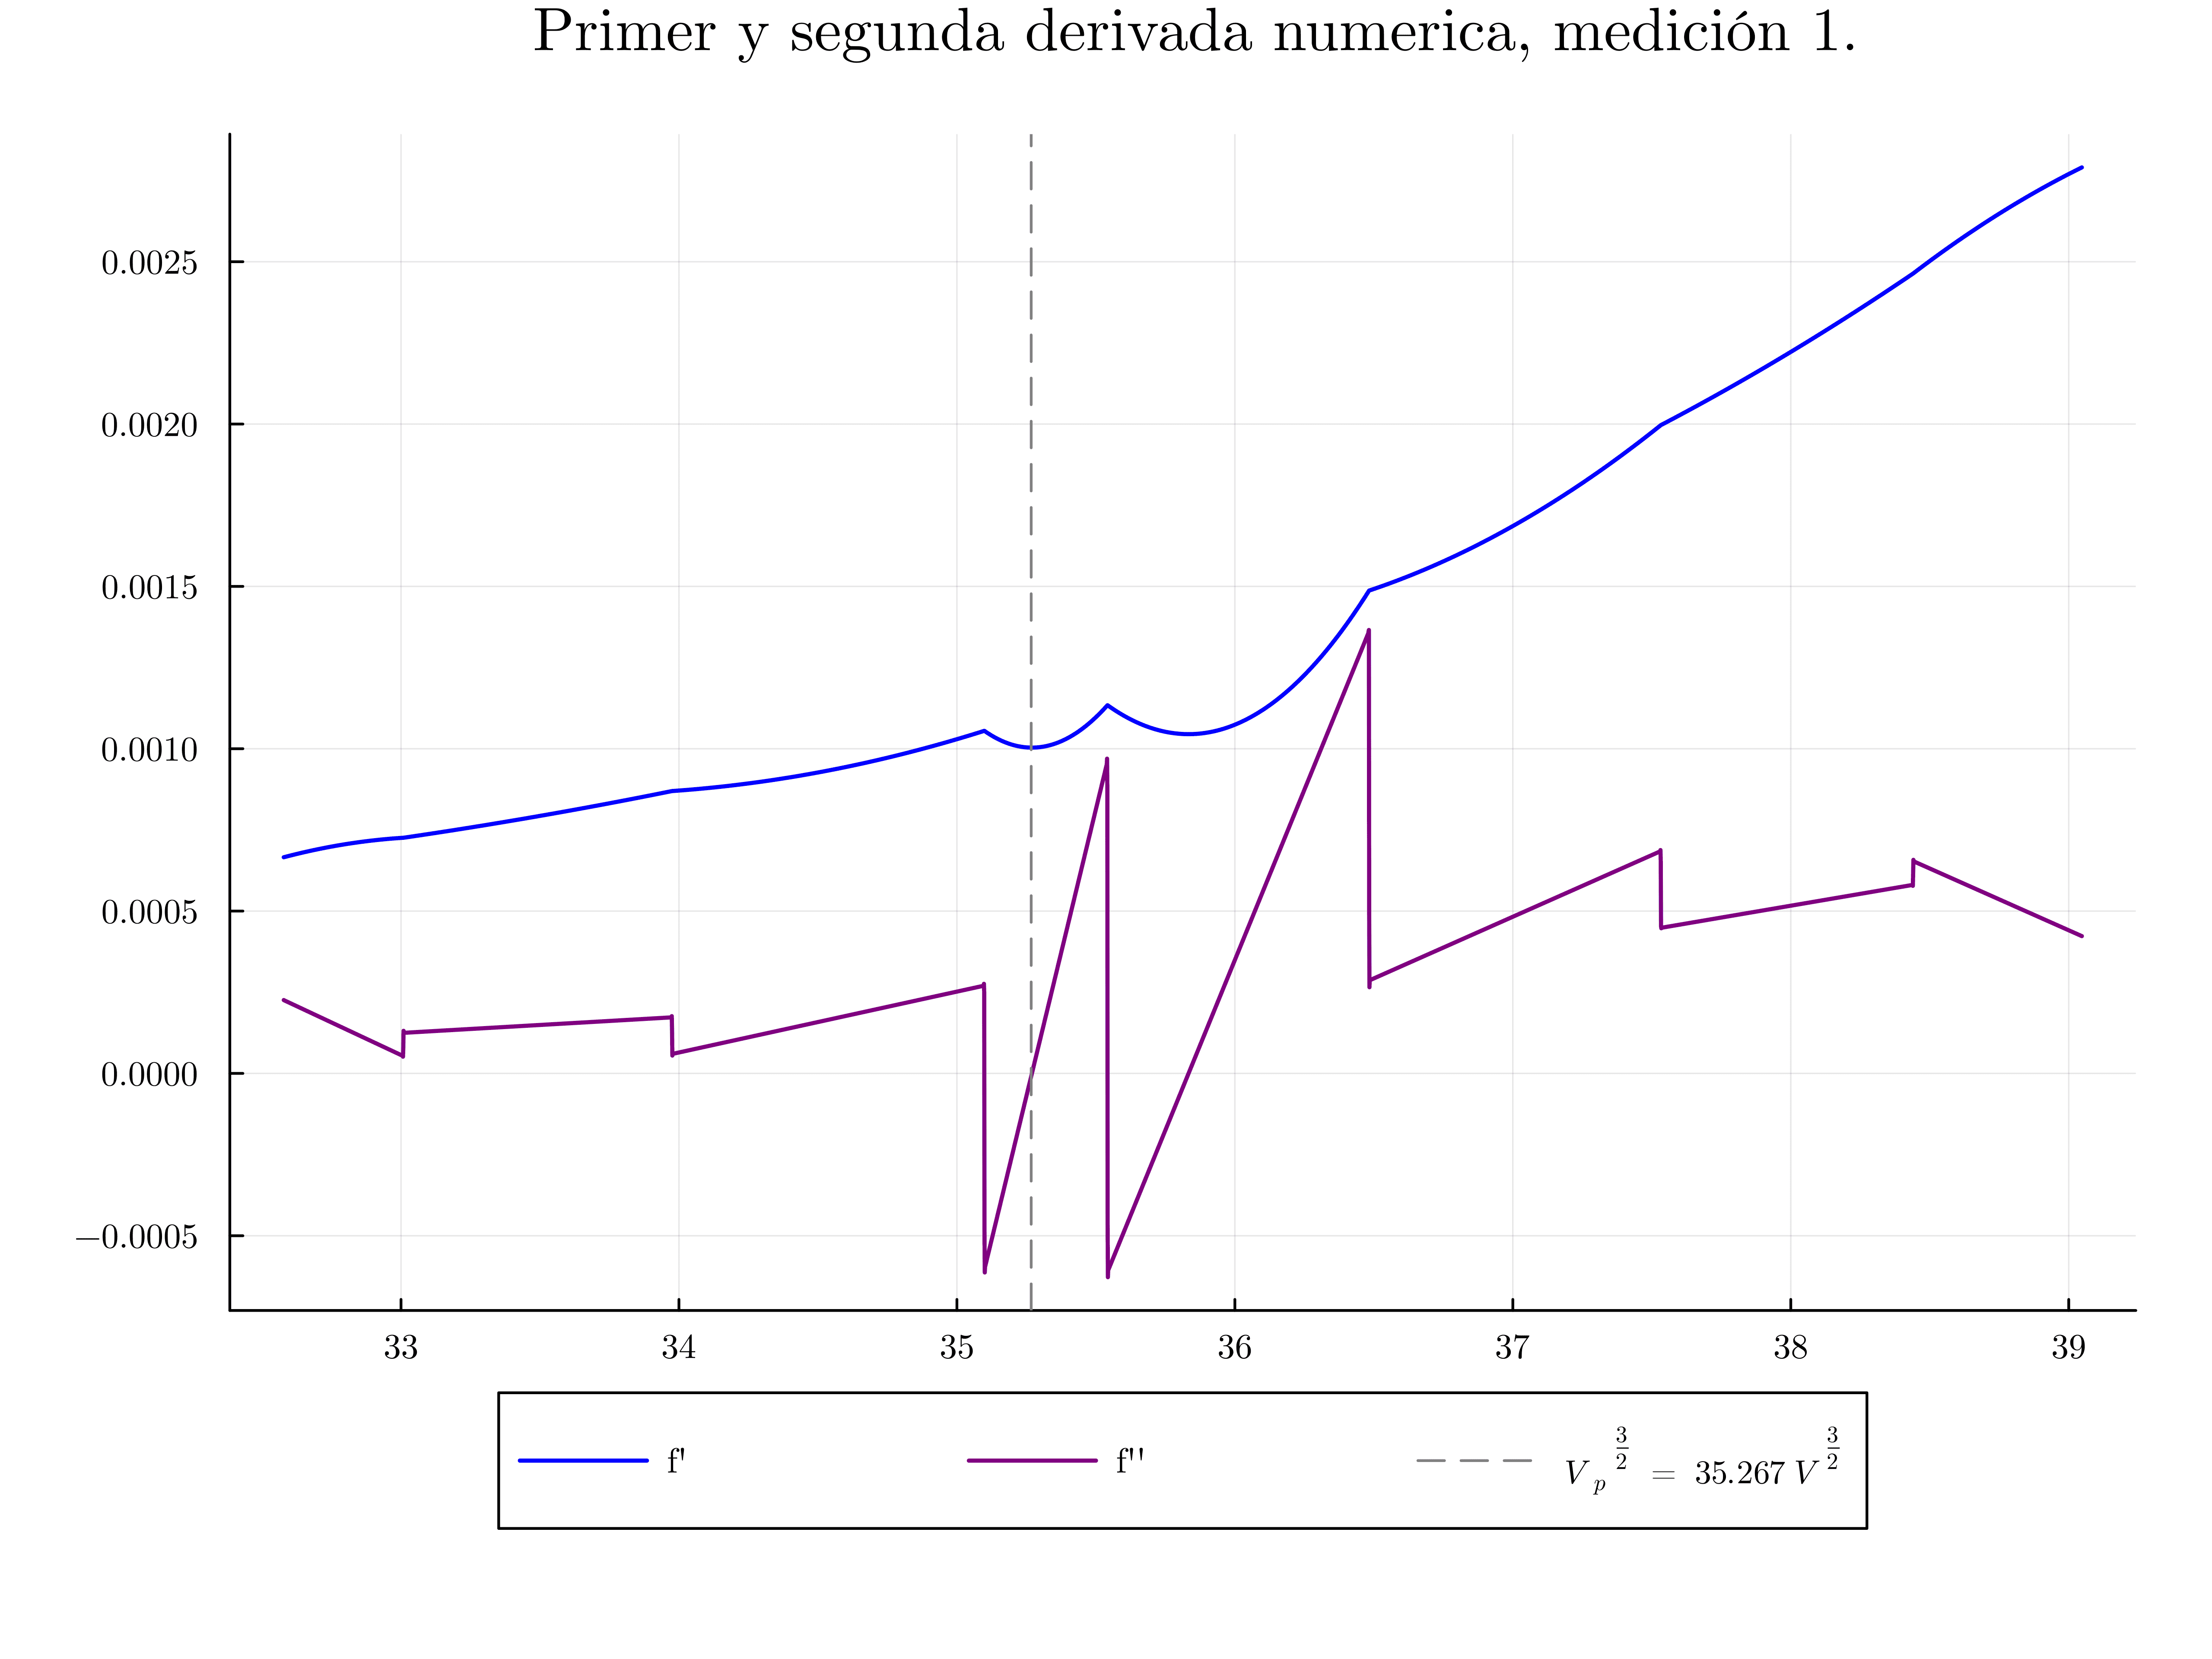
\includegraphics[width=\linewidth]{img/potderps1.png}
	\caption{Barrido n°: 1}
	\label{fig:potderps1}
\end{subfigure}
\hfill
\begin{subfigure}[b]{0.49\textwidth}
	\centering
	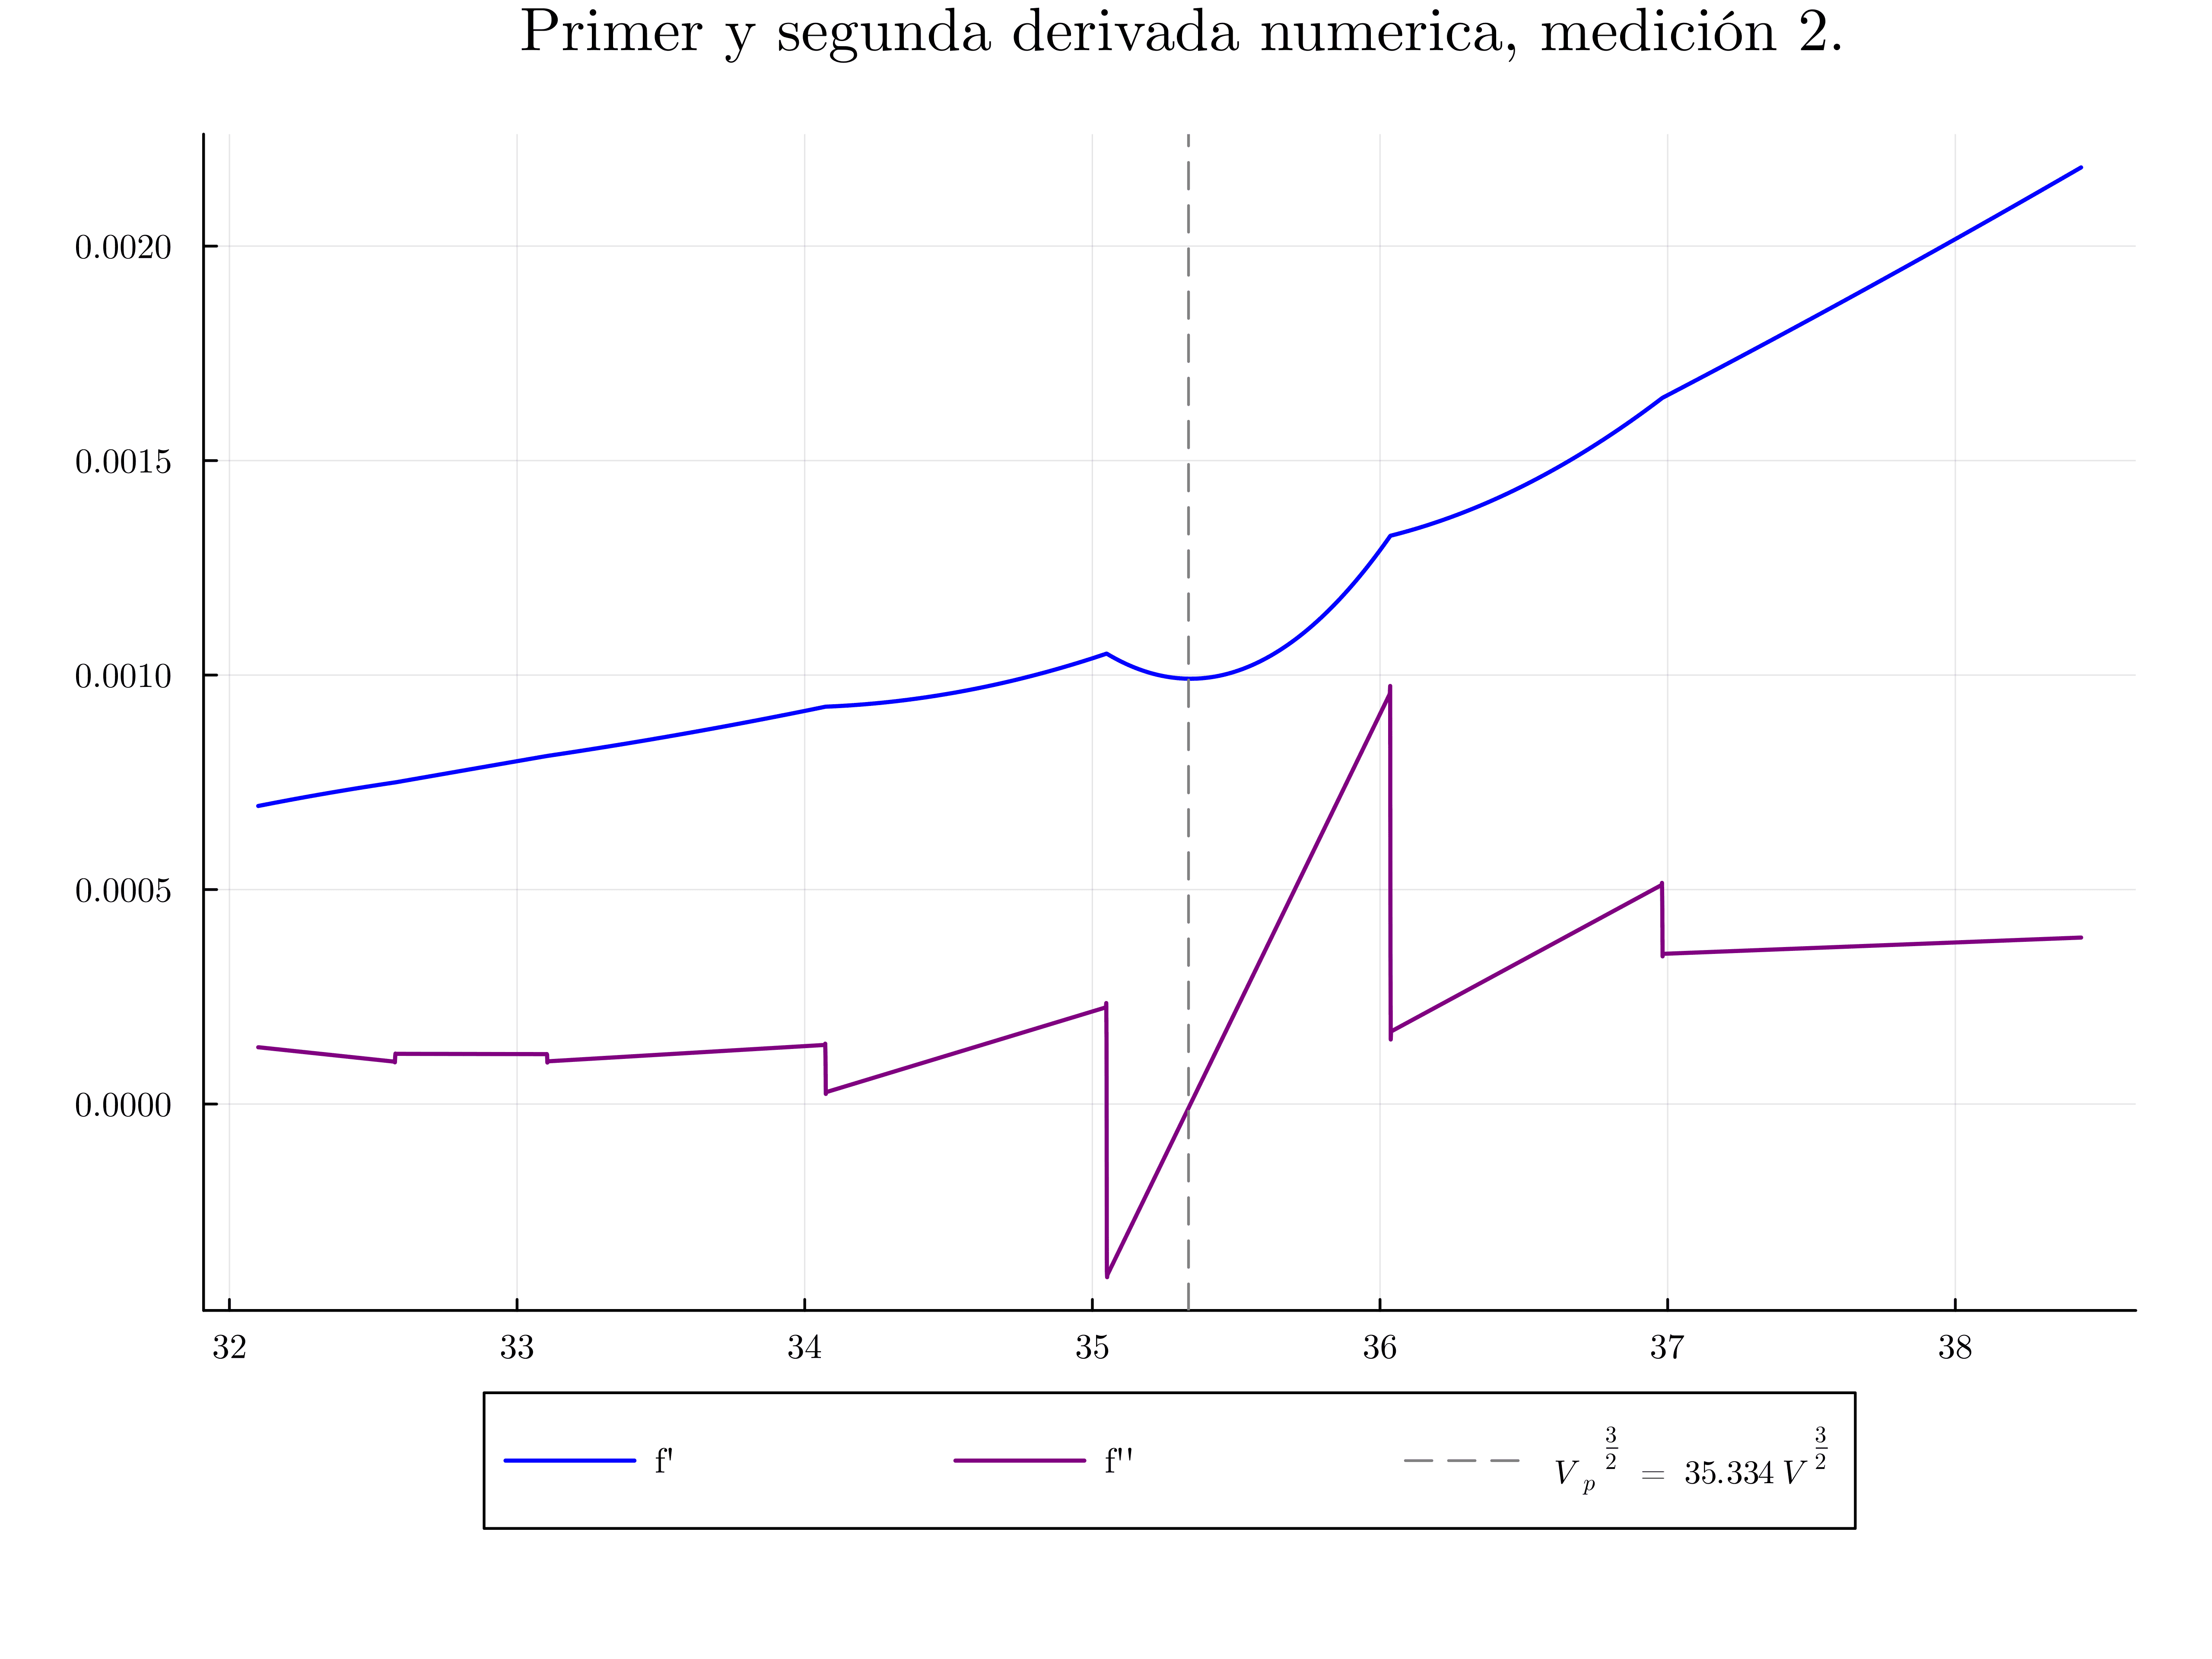
\includegraphics[width=\linewidth]{img/potderps2.png}
	\caption{Barrido n°: 2}
	\label{fig:potderps2}
\end{subfigure}

\end{figure}

% segundo bloque de figuras
\begin{figure}[H]
\ContinuedFloat
\centering
\begin{subfigure}[b]{0.49\textwidth}
	\centering
	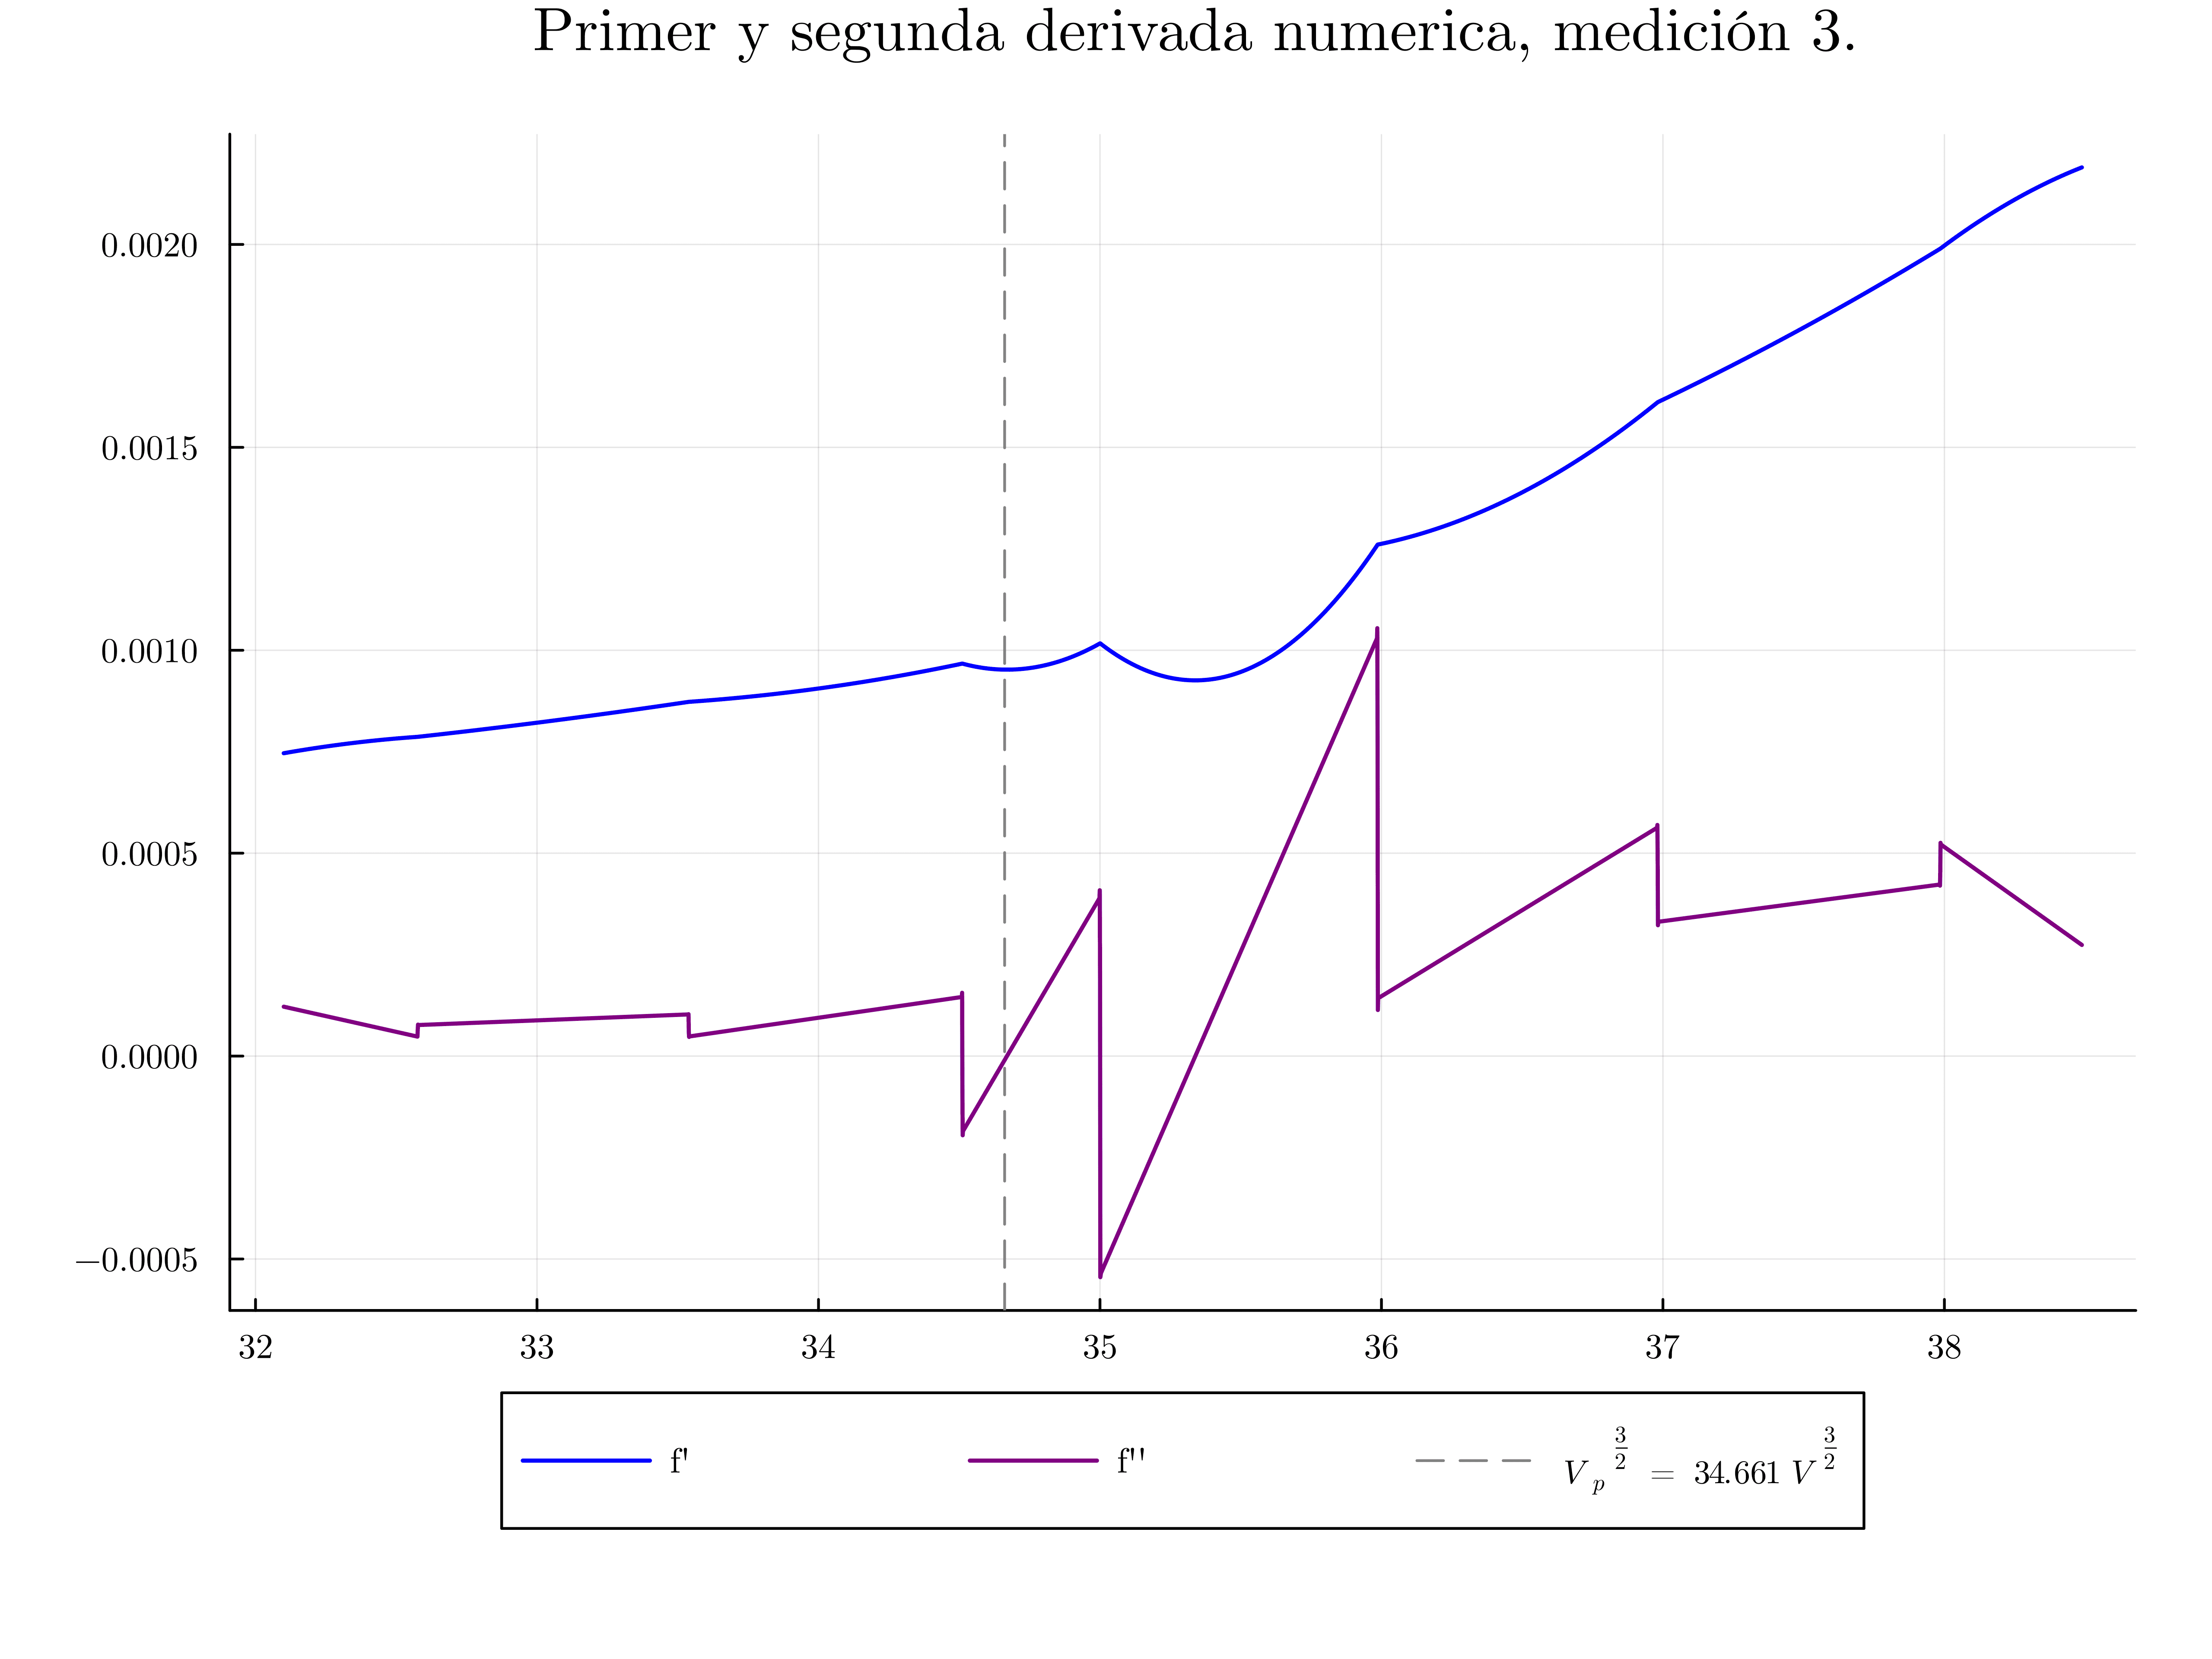
\includegraphics[width=\linewidth]{img/potderps3.png}
	\caption{Barrido n°: 3}
	\label{fig:potderps3}
\end{subfigure}
\hfill
\begin{subfigure}[b]{0.49\textwidth}
	\centering
	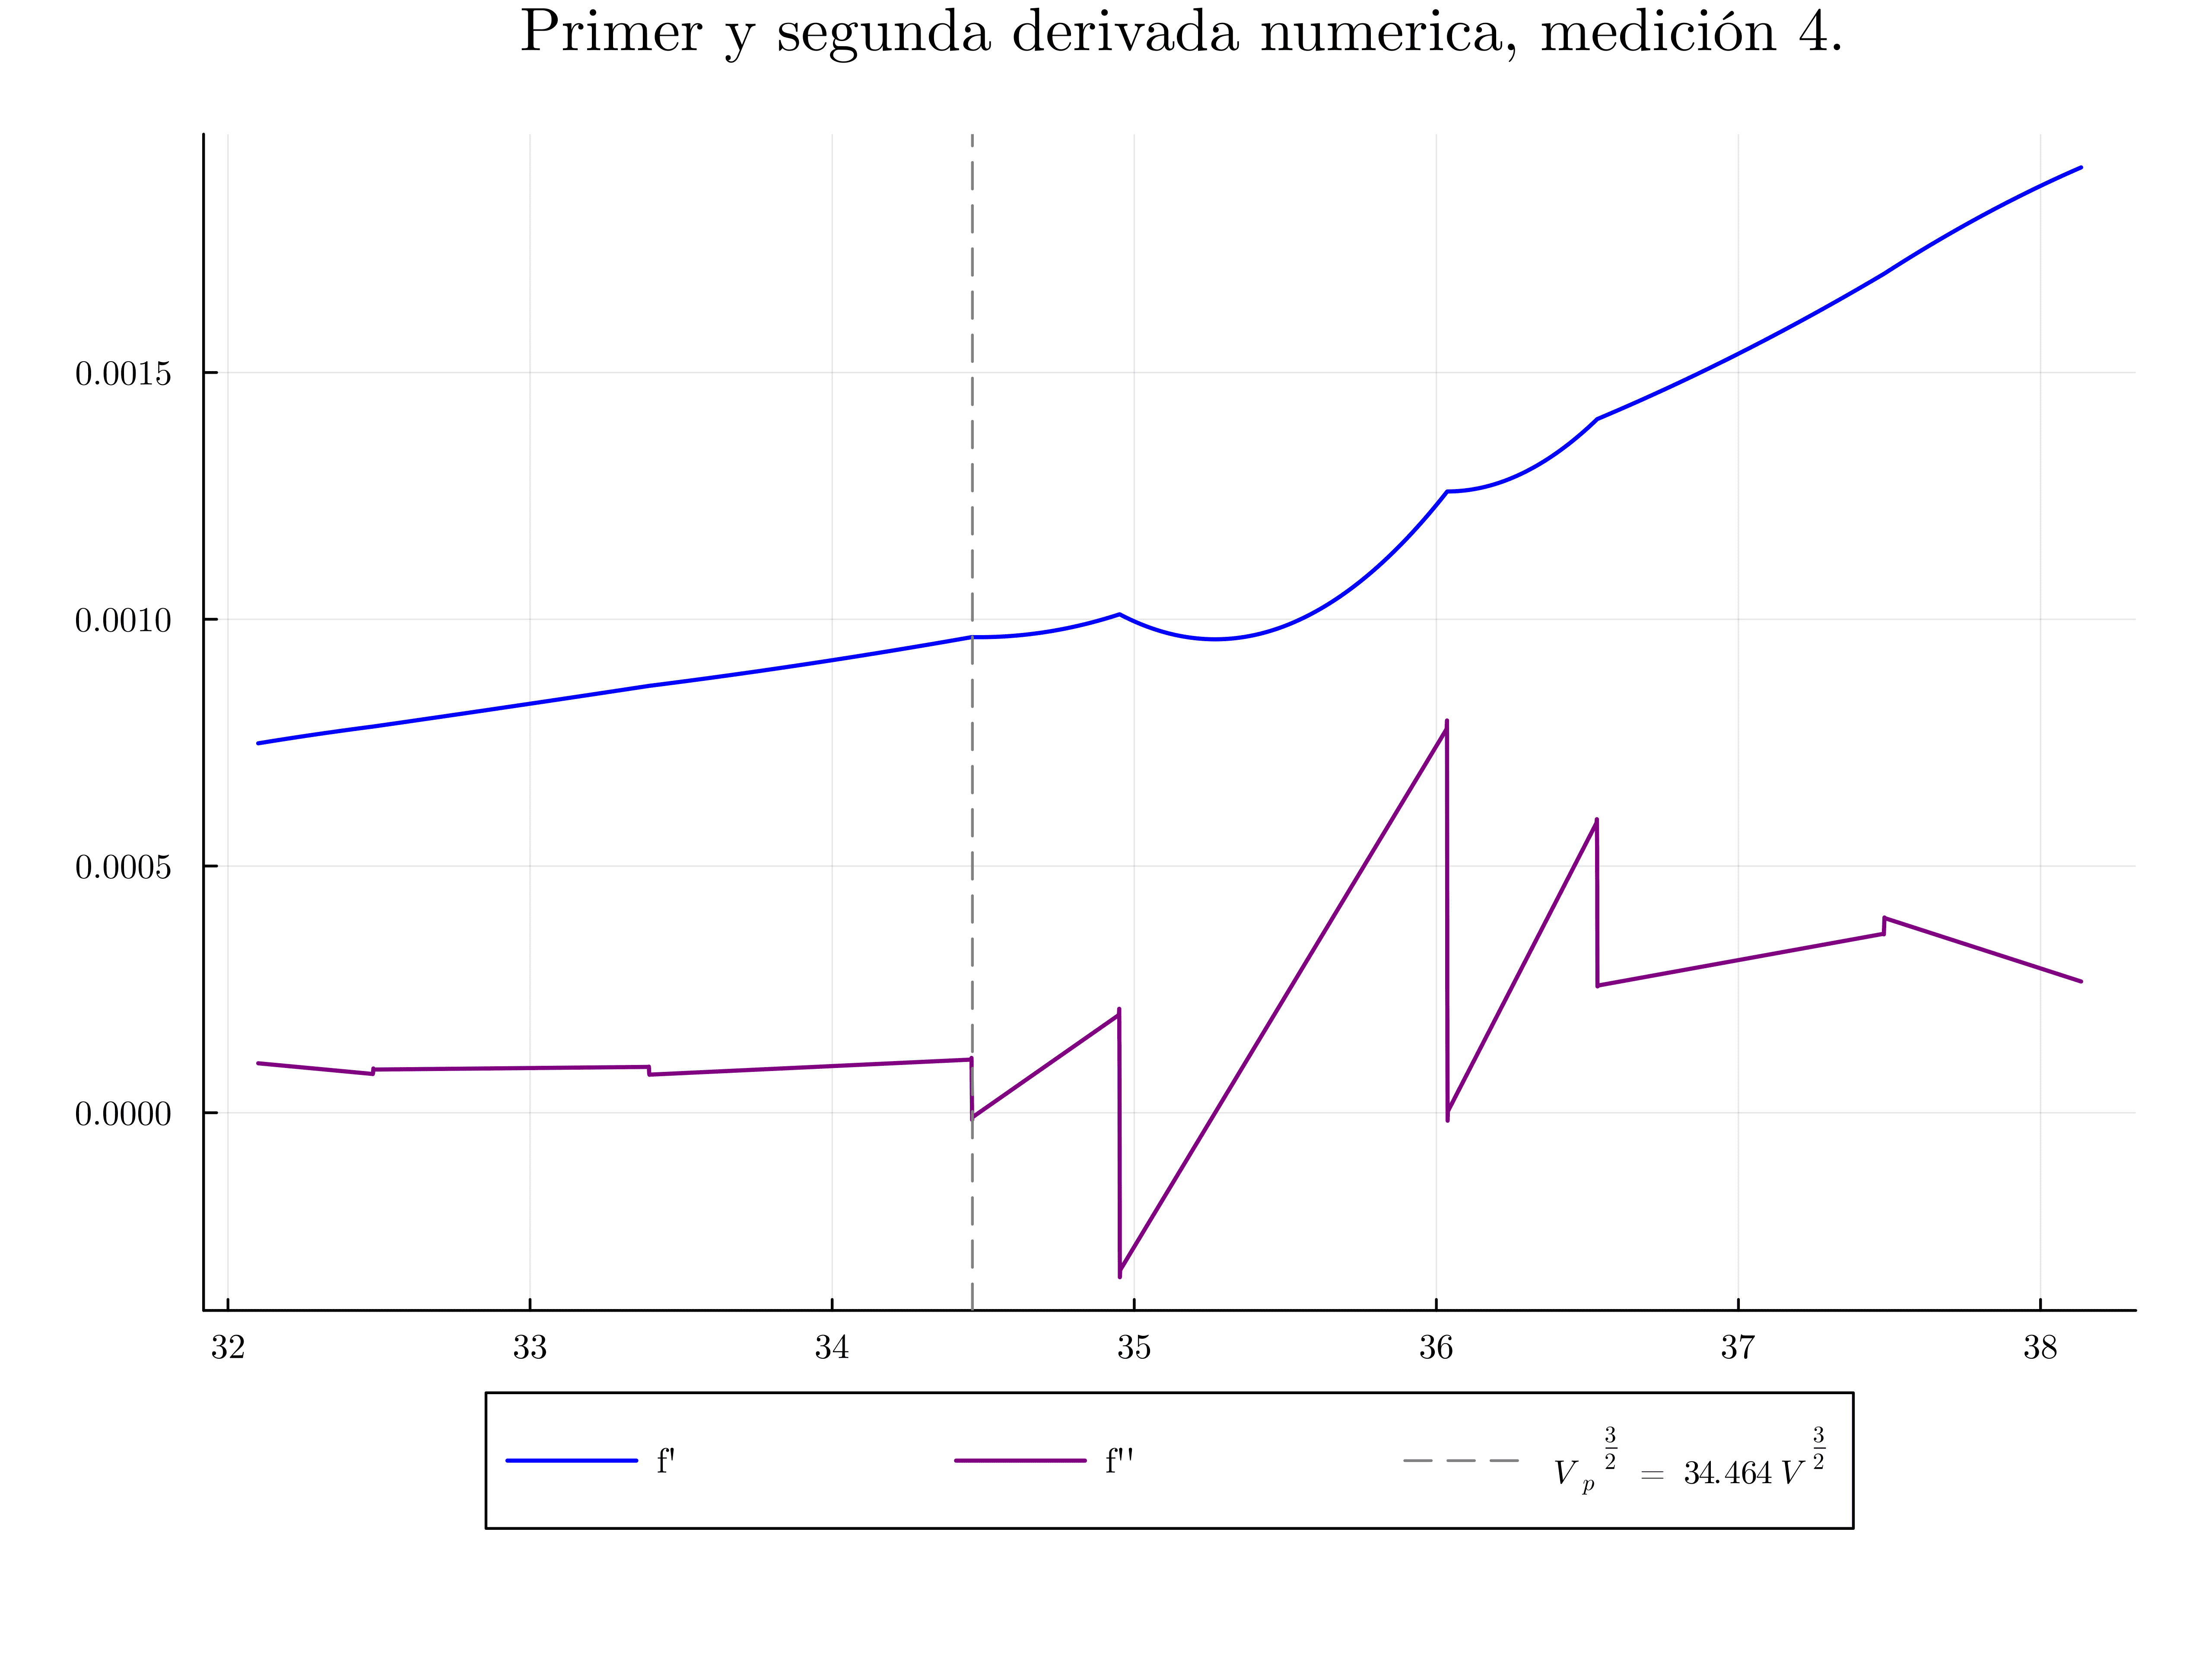
\includegraphics[width=\linewidth]{img/potderps4.png}
	\caption{Barrido n°: 4}
	\label{fig:potderps4}
\end{subfigure}

\end{figure}

% teercer bloque de figuras
\begin{figure}[H]
\ContinuedFloat % Indica que esta figura continúa de la anterior
\centering
\begin{subfigure}[b]{0.49\textwidth}
	\centering
	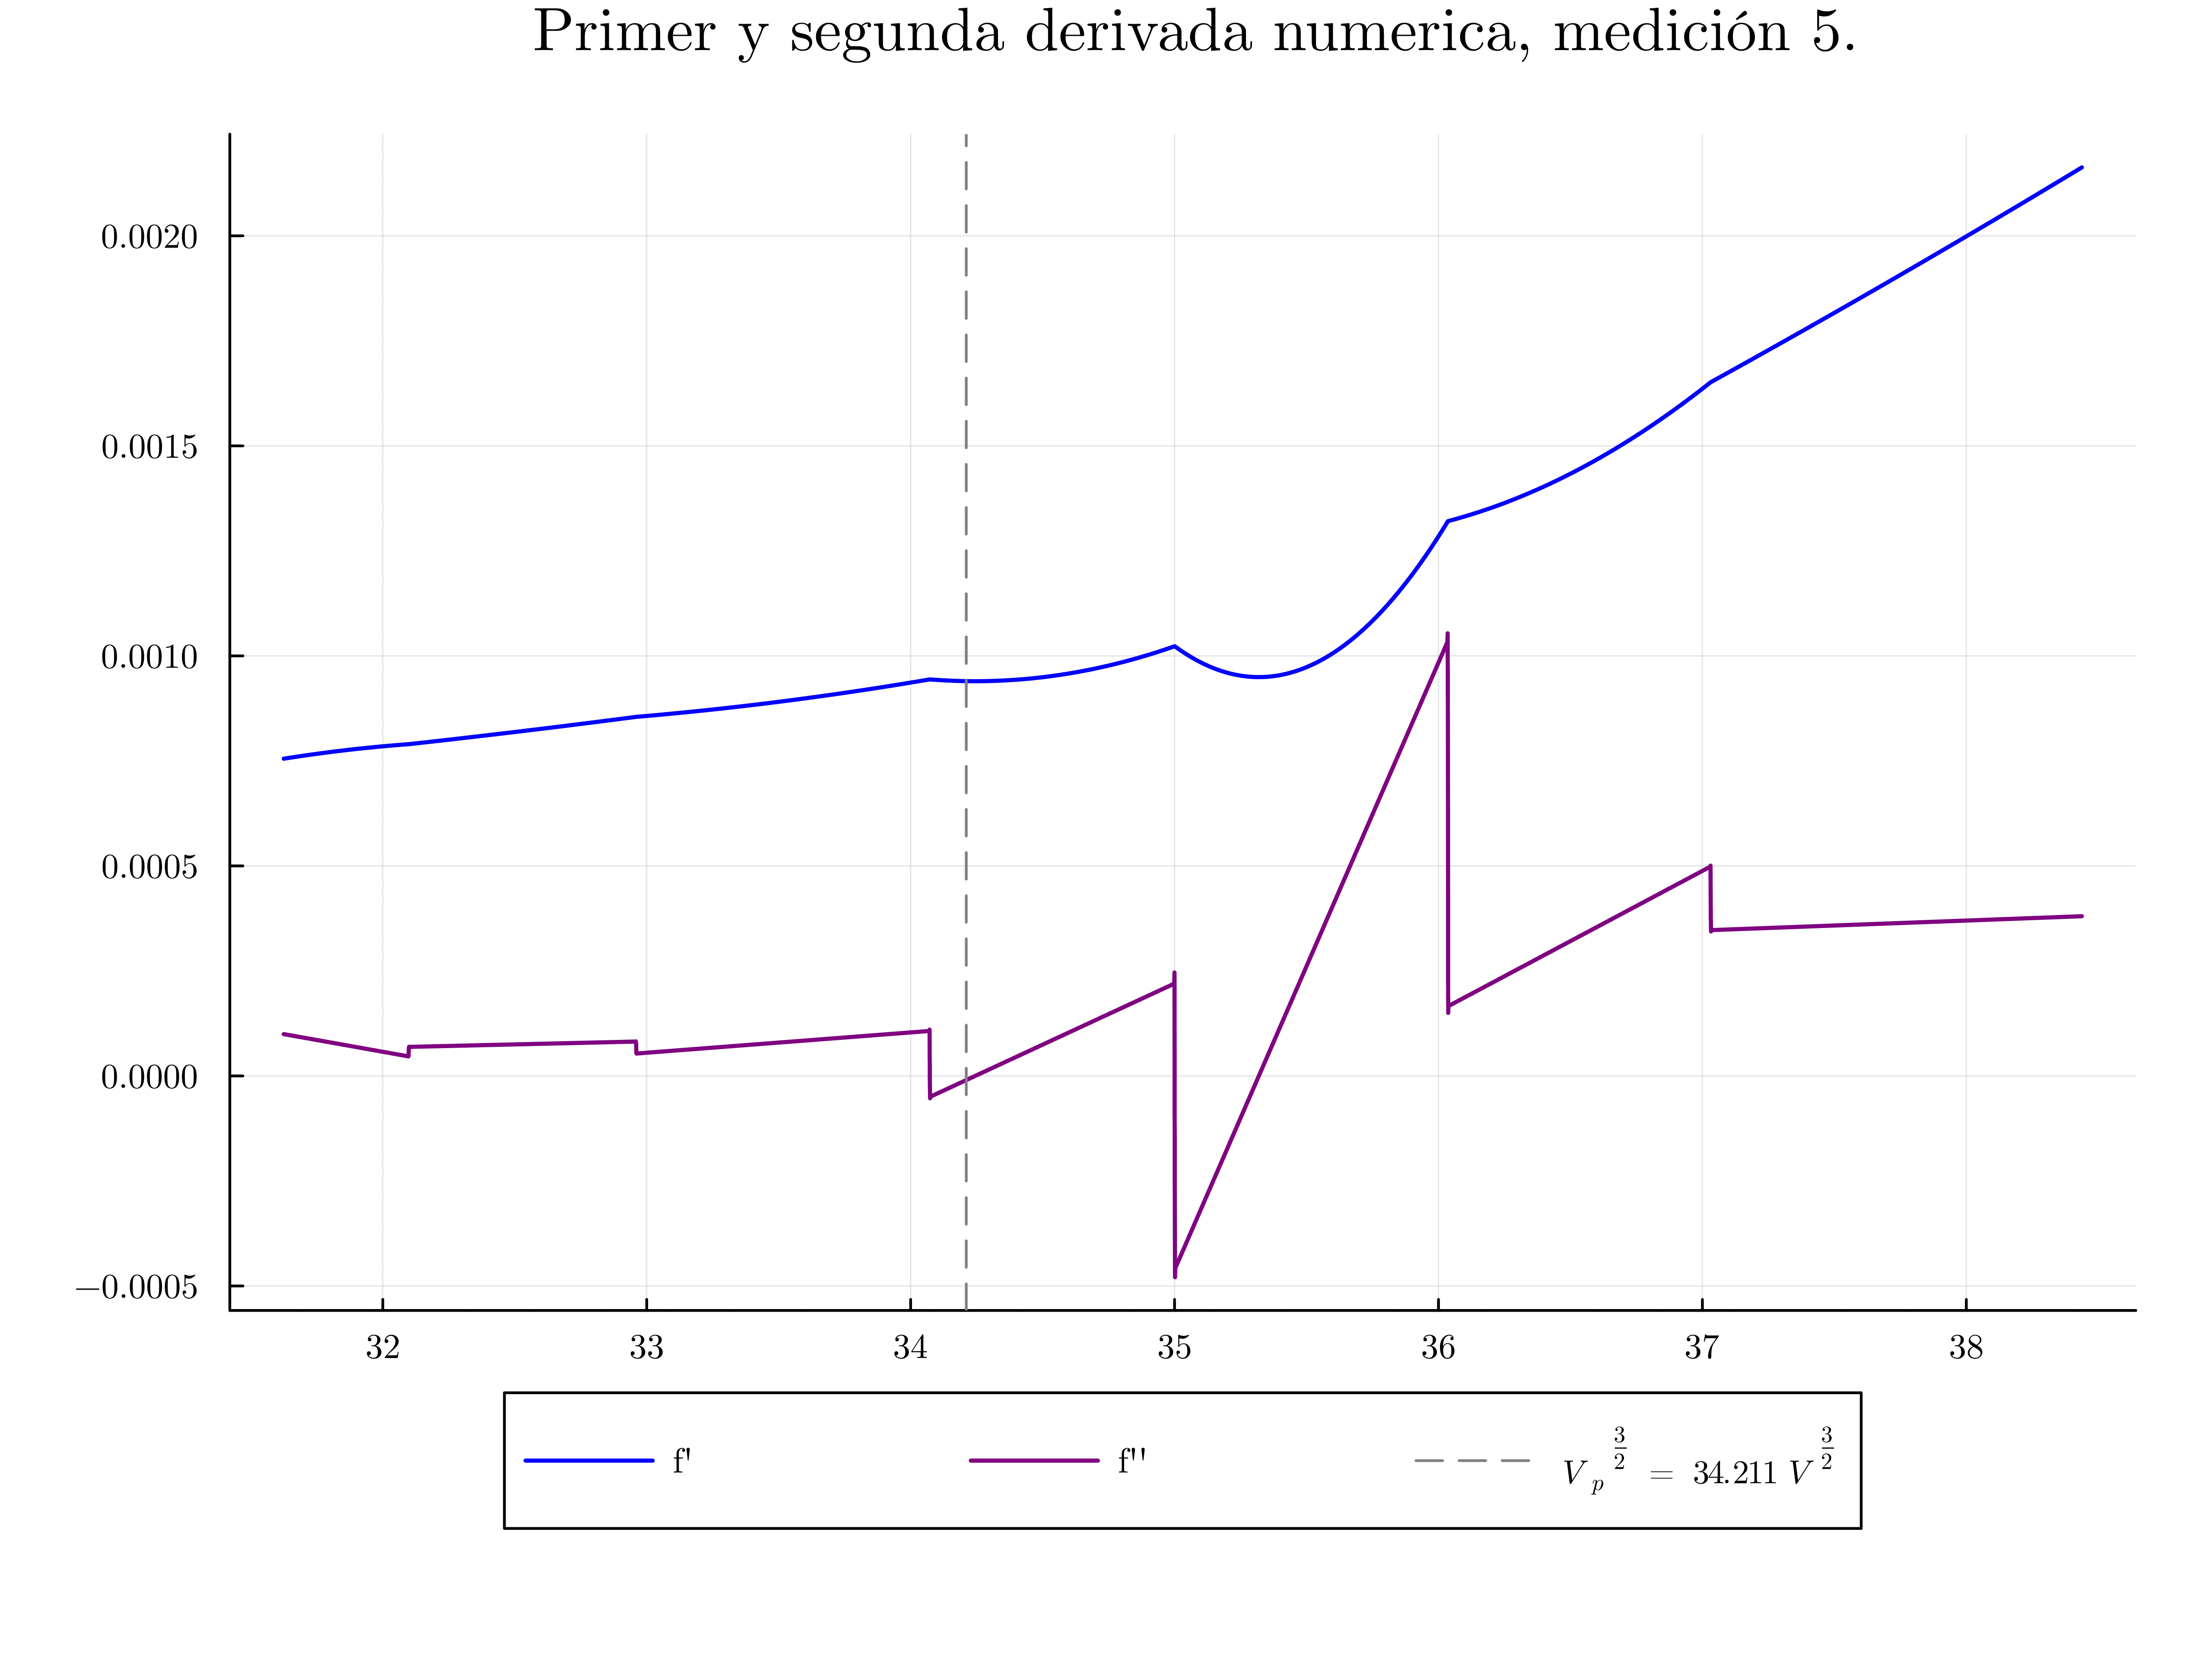
\includegraphics[width=\linewidth]{img/potderps5.png}
	\caption{Barrido n°: 5}
	\label{fig:potderps5}
\end{subfigure}
\hfill
\begin{subfigure}[b]{0.49\textwidth}
	\centering
	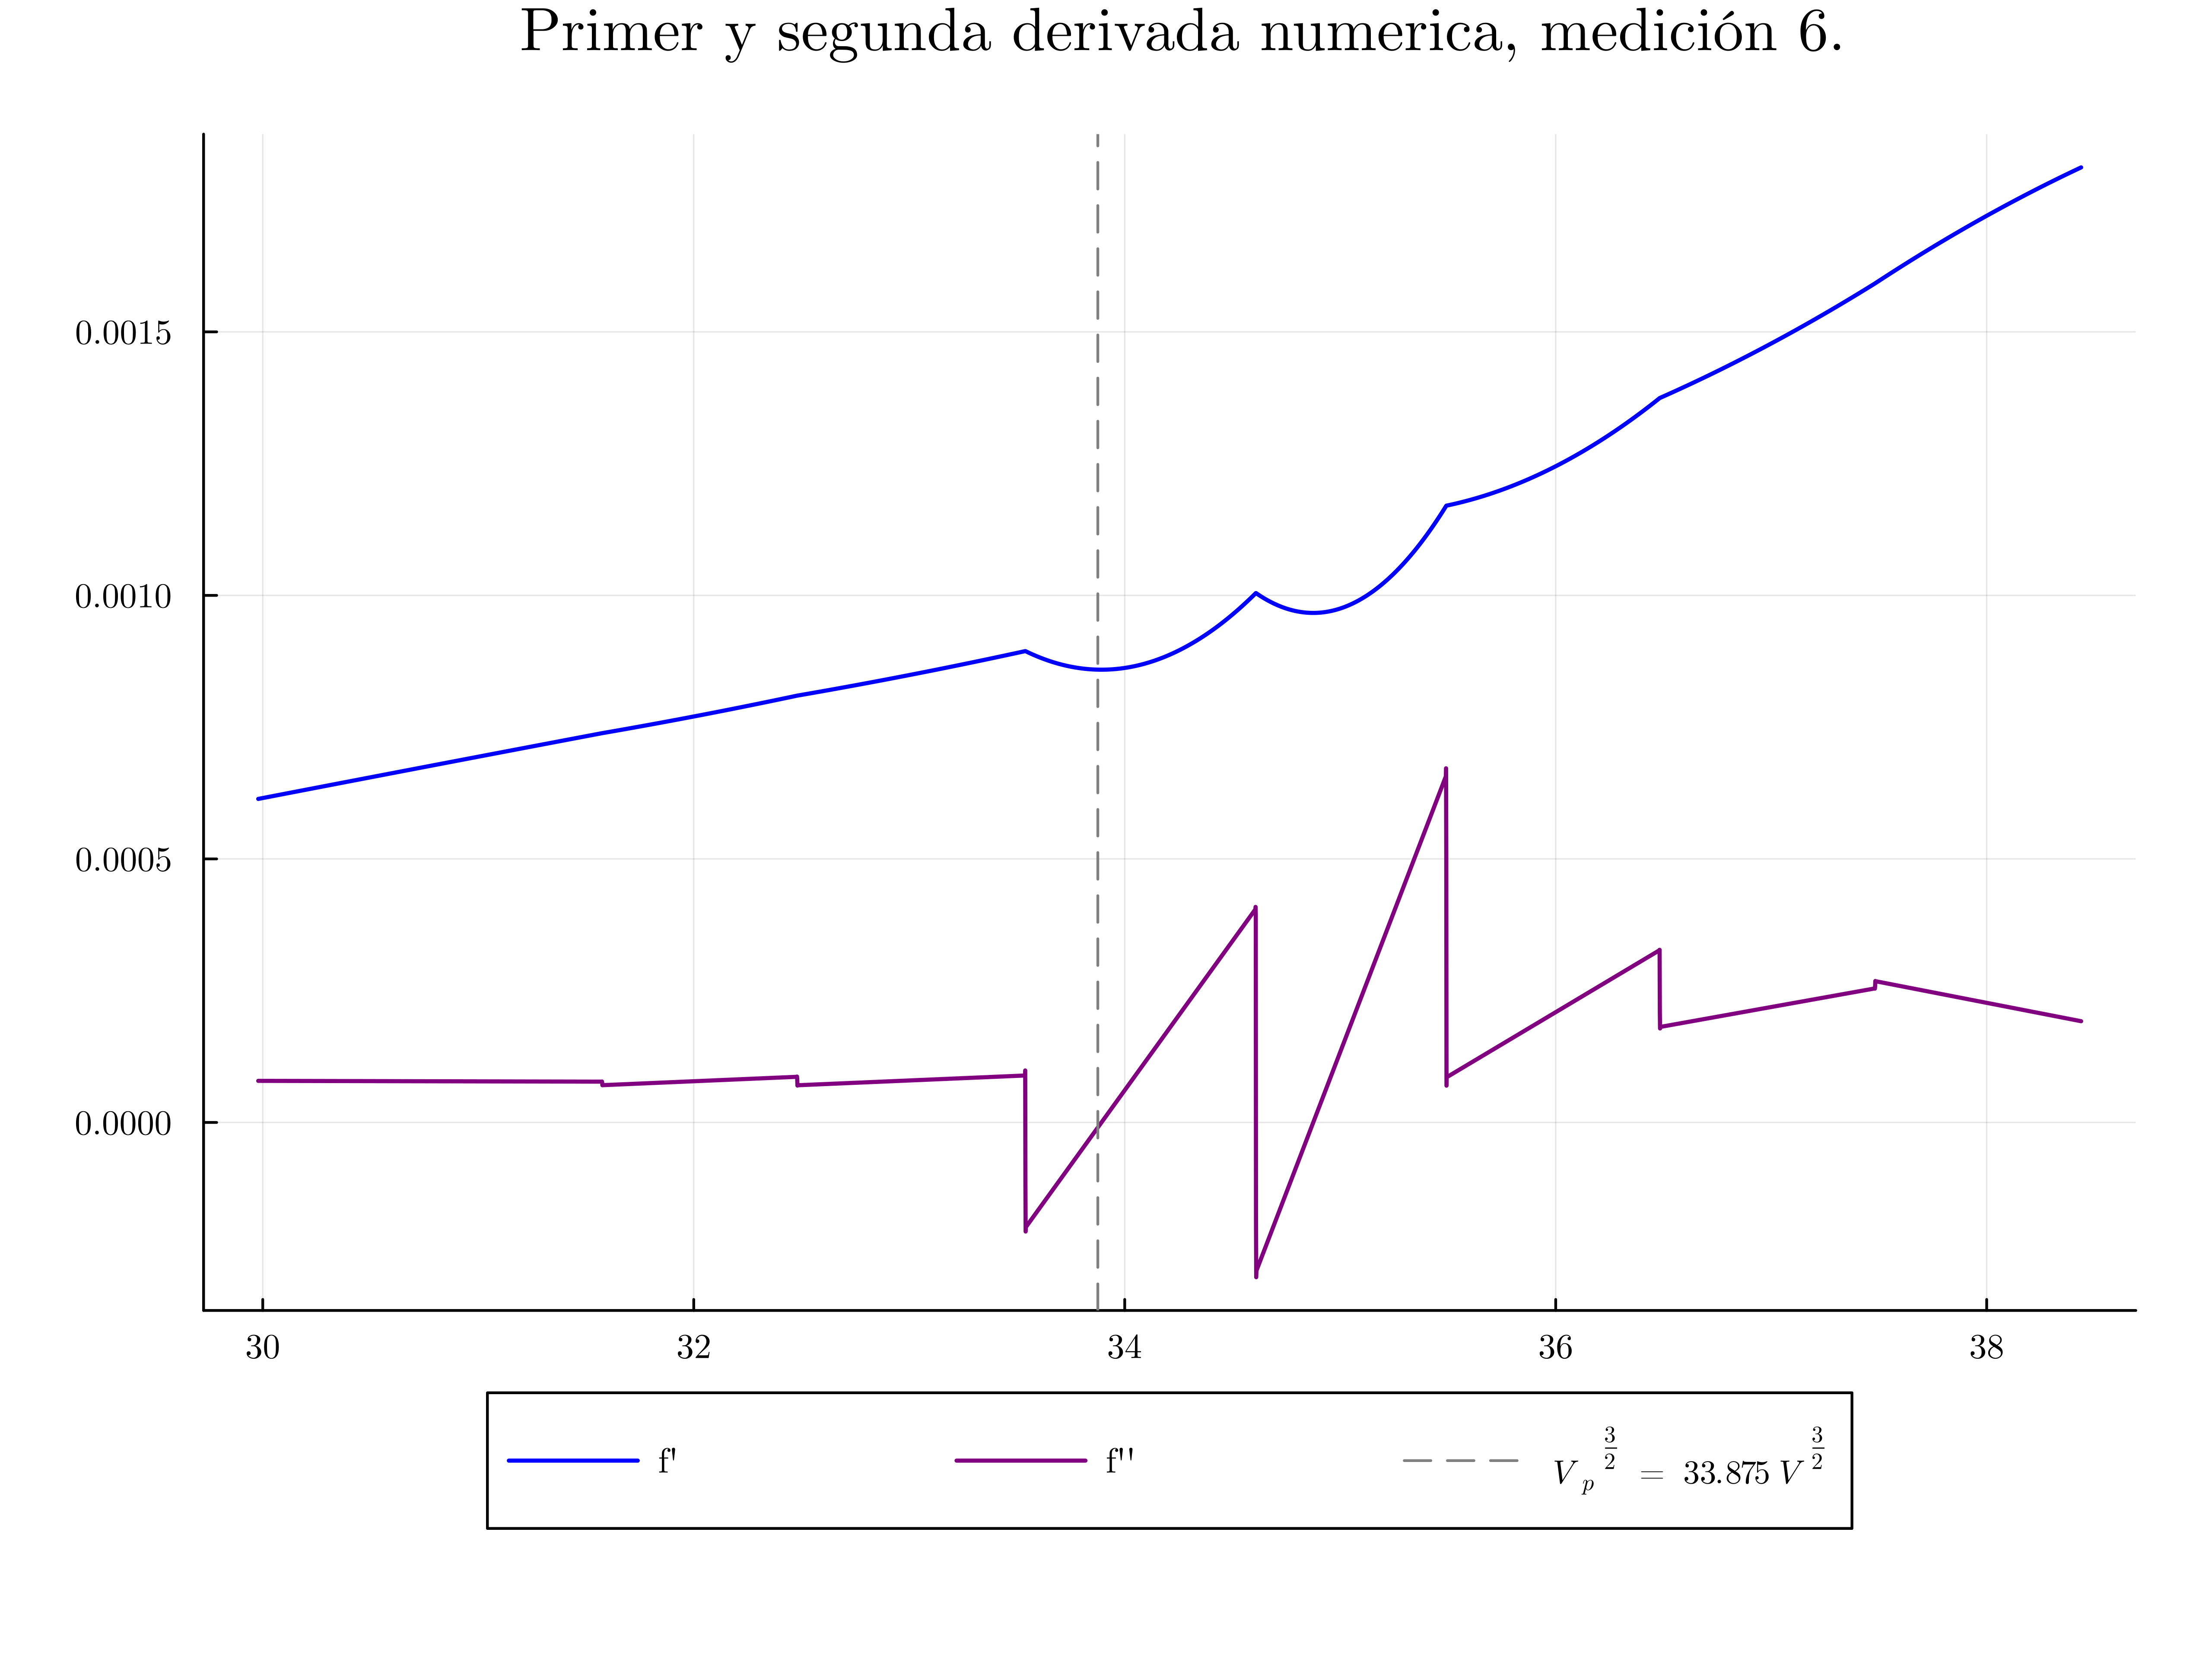
\includegraphics[width=\linewidth]{img/potderps6.png}
	\caption{Barrido n°: 6}
	\label{fig:potderps6}
\end{subfigure}

\end{figure}

% cuarto bloque de figuras
\begin{figure}[H]
\ContinuedFloat % Indica que esta figura continúa de la anterior
\centering
\begin{subfigure}[b]{0.49\textwidth}
	\centering
	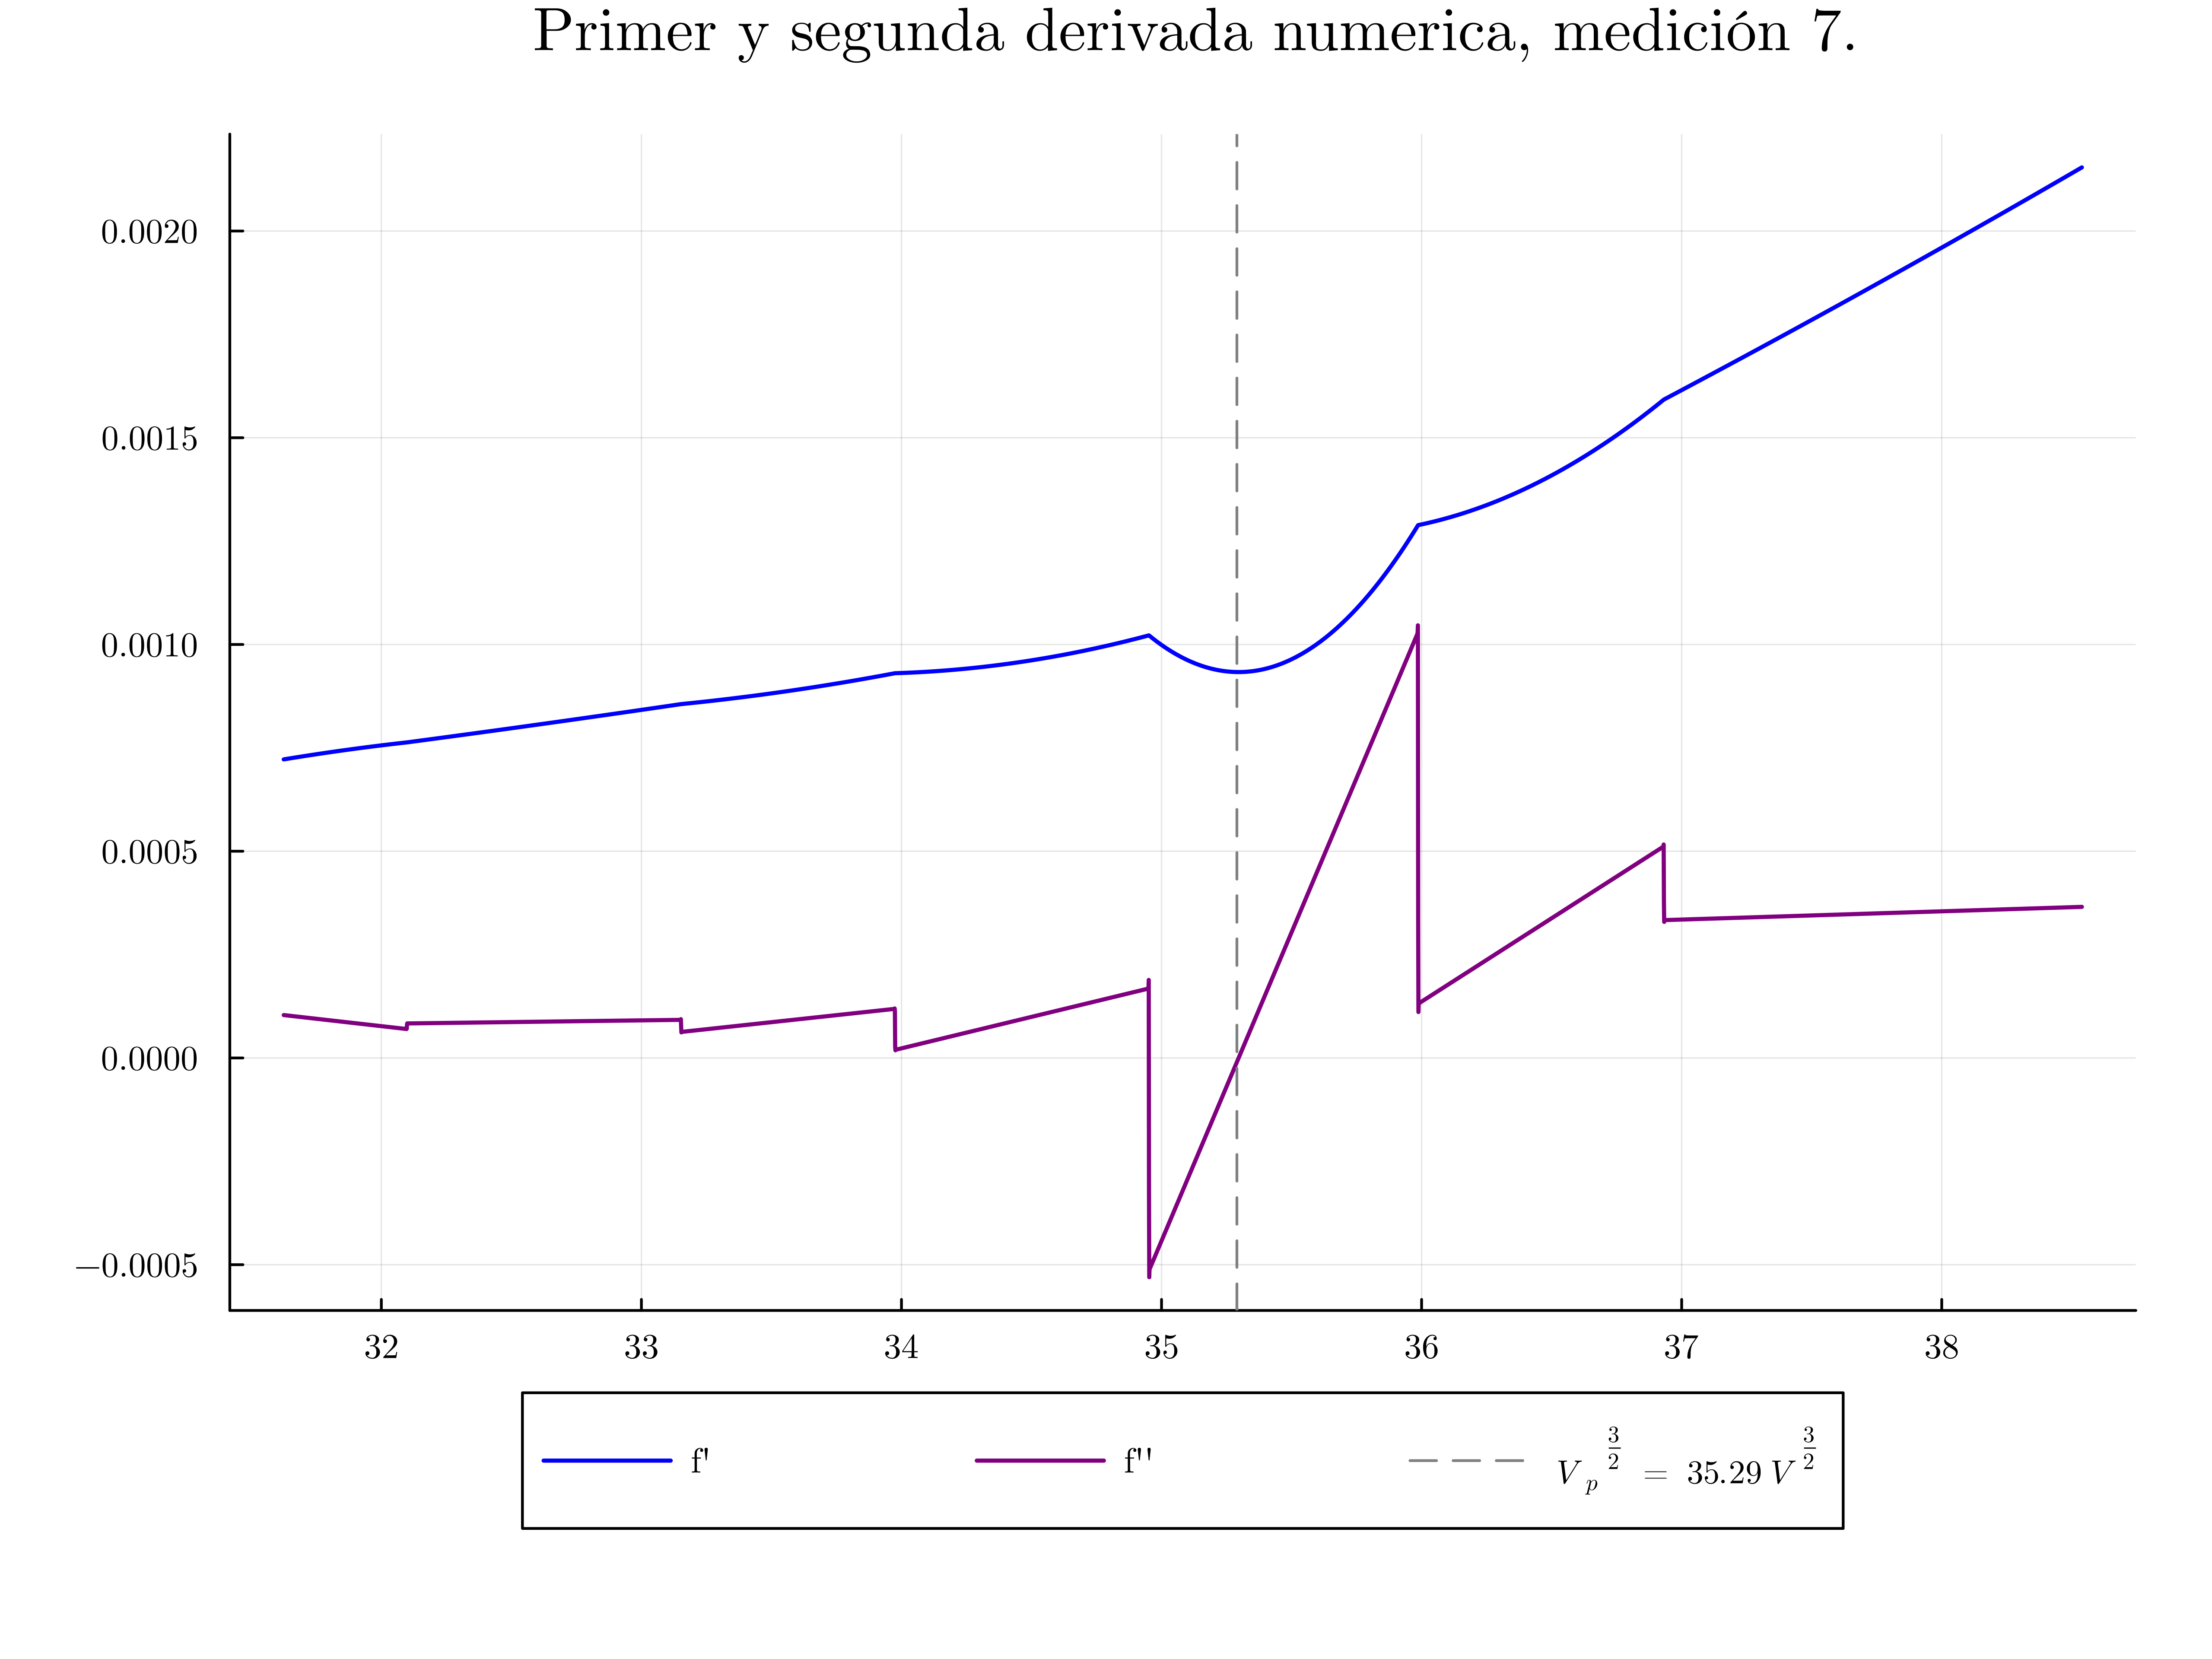
\includegraphics[width=\linewidth]{img/potderps7.png}
	\caption{Barrido n°: 7}
	\label{fig:potderps7}
\end{subfigure}
\hfill
\begin{subfigure}[b]{0.49\textwidth}
	\centering
	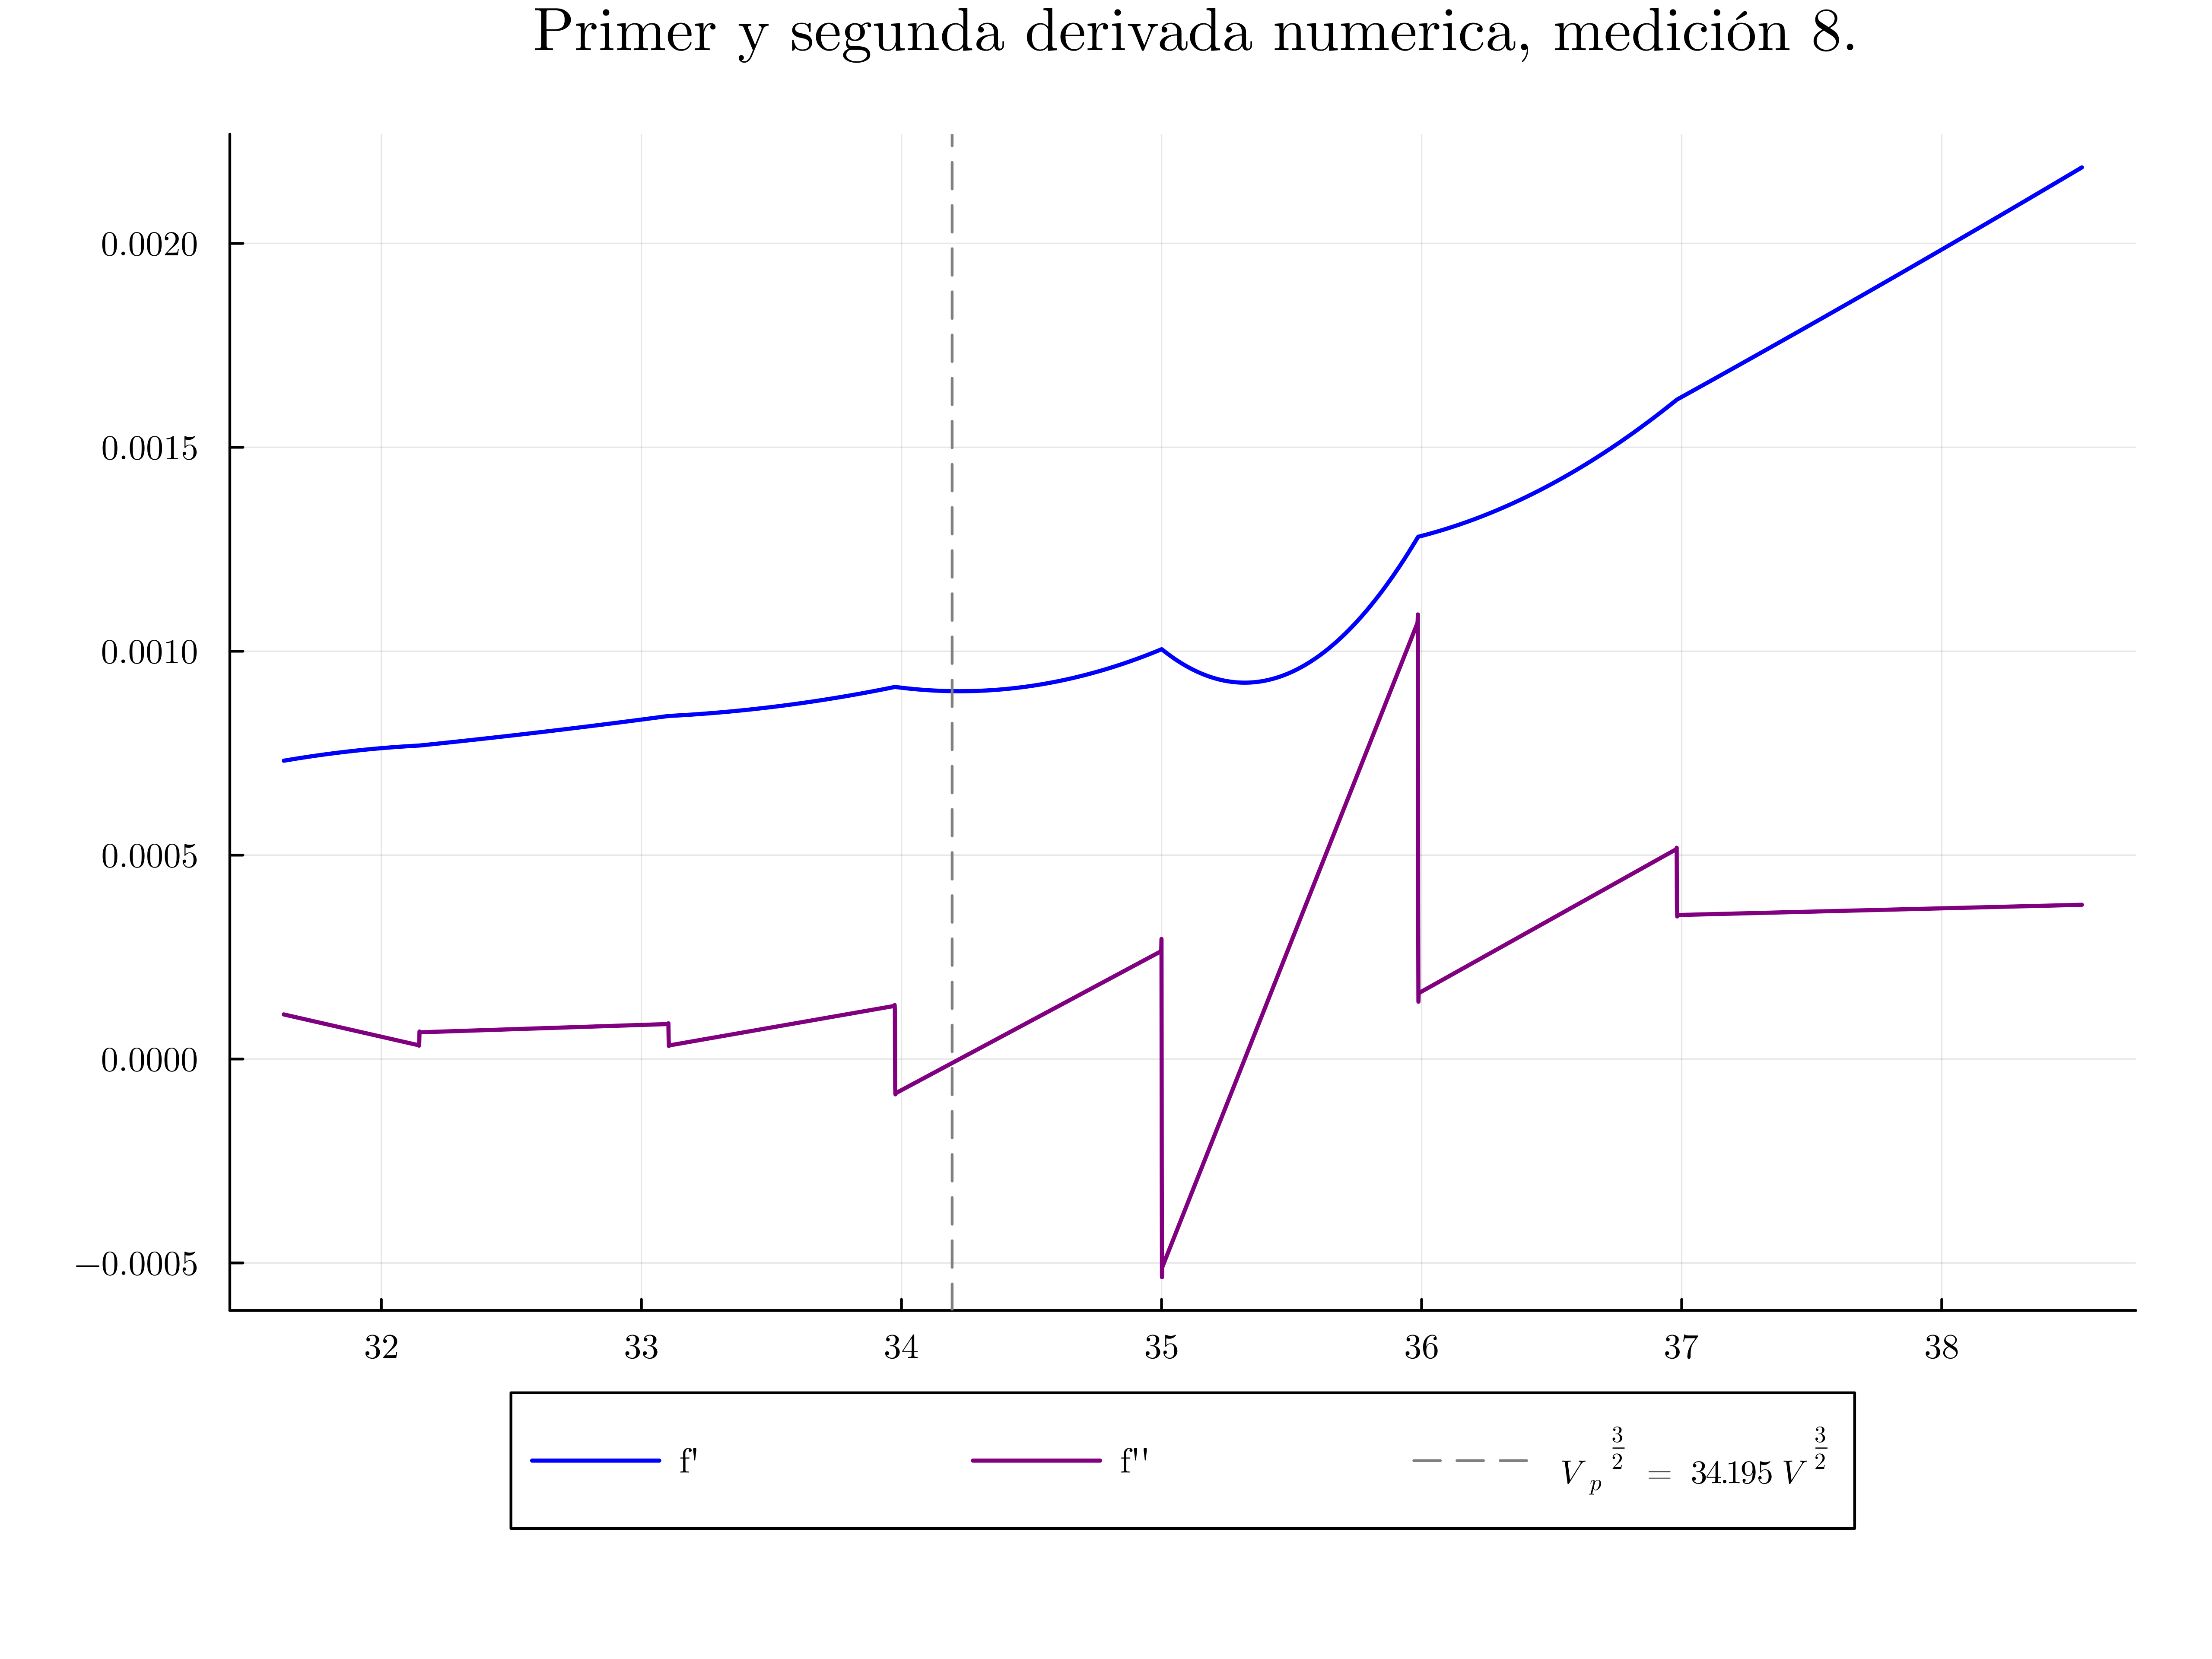
\includegraphics[width=\linewidth]{img/potderps8.png}
	\caption{Barrido n°: 8}
	\label{fig:potderps8}
\end{subfigure}
\end{figure}


% Últimas figuras
\begin{figure}[H]
\ContinuedFloat % Sigue con la misma numeración y caption
\centering
\begin{subfigure}[b]{0.49\textwidth}
	\centering
	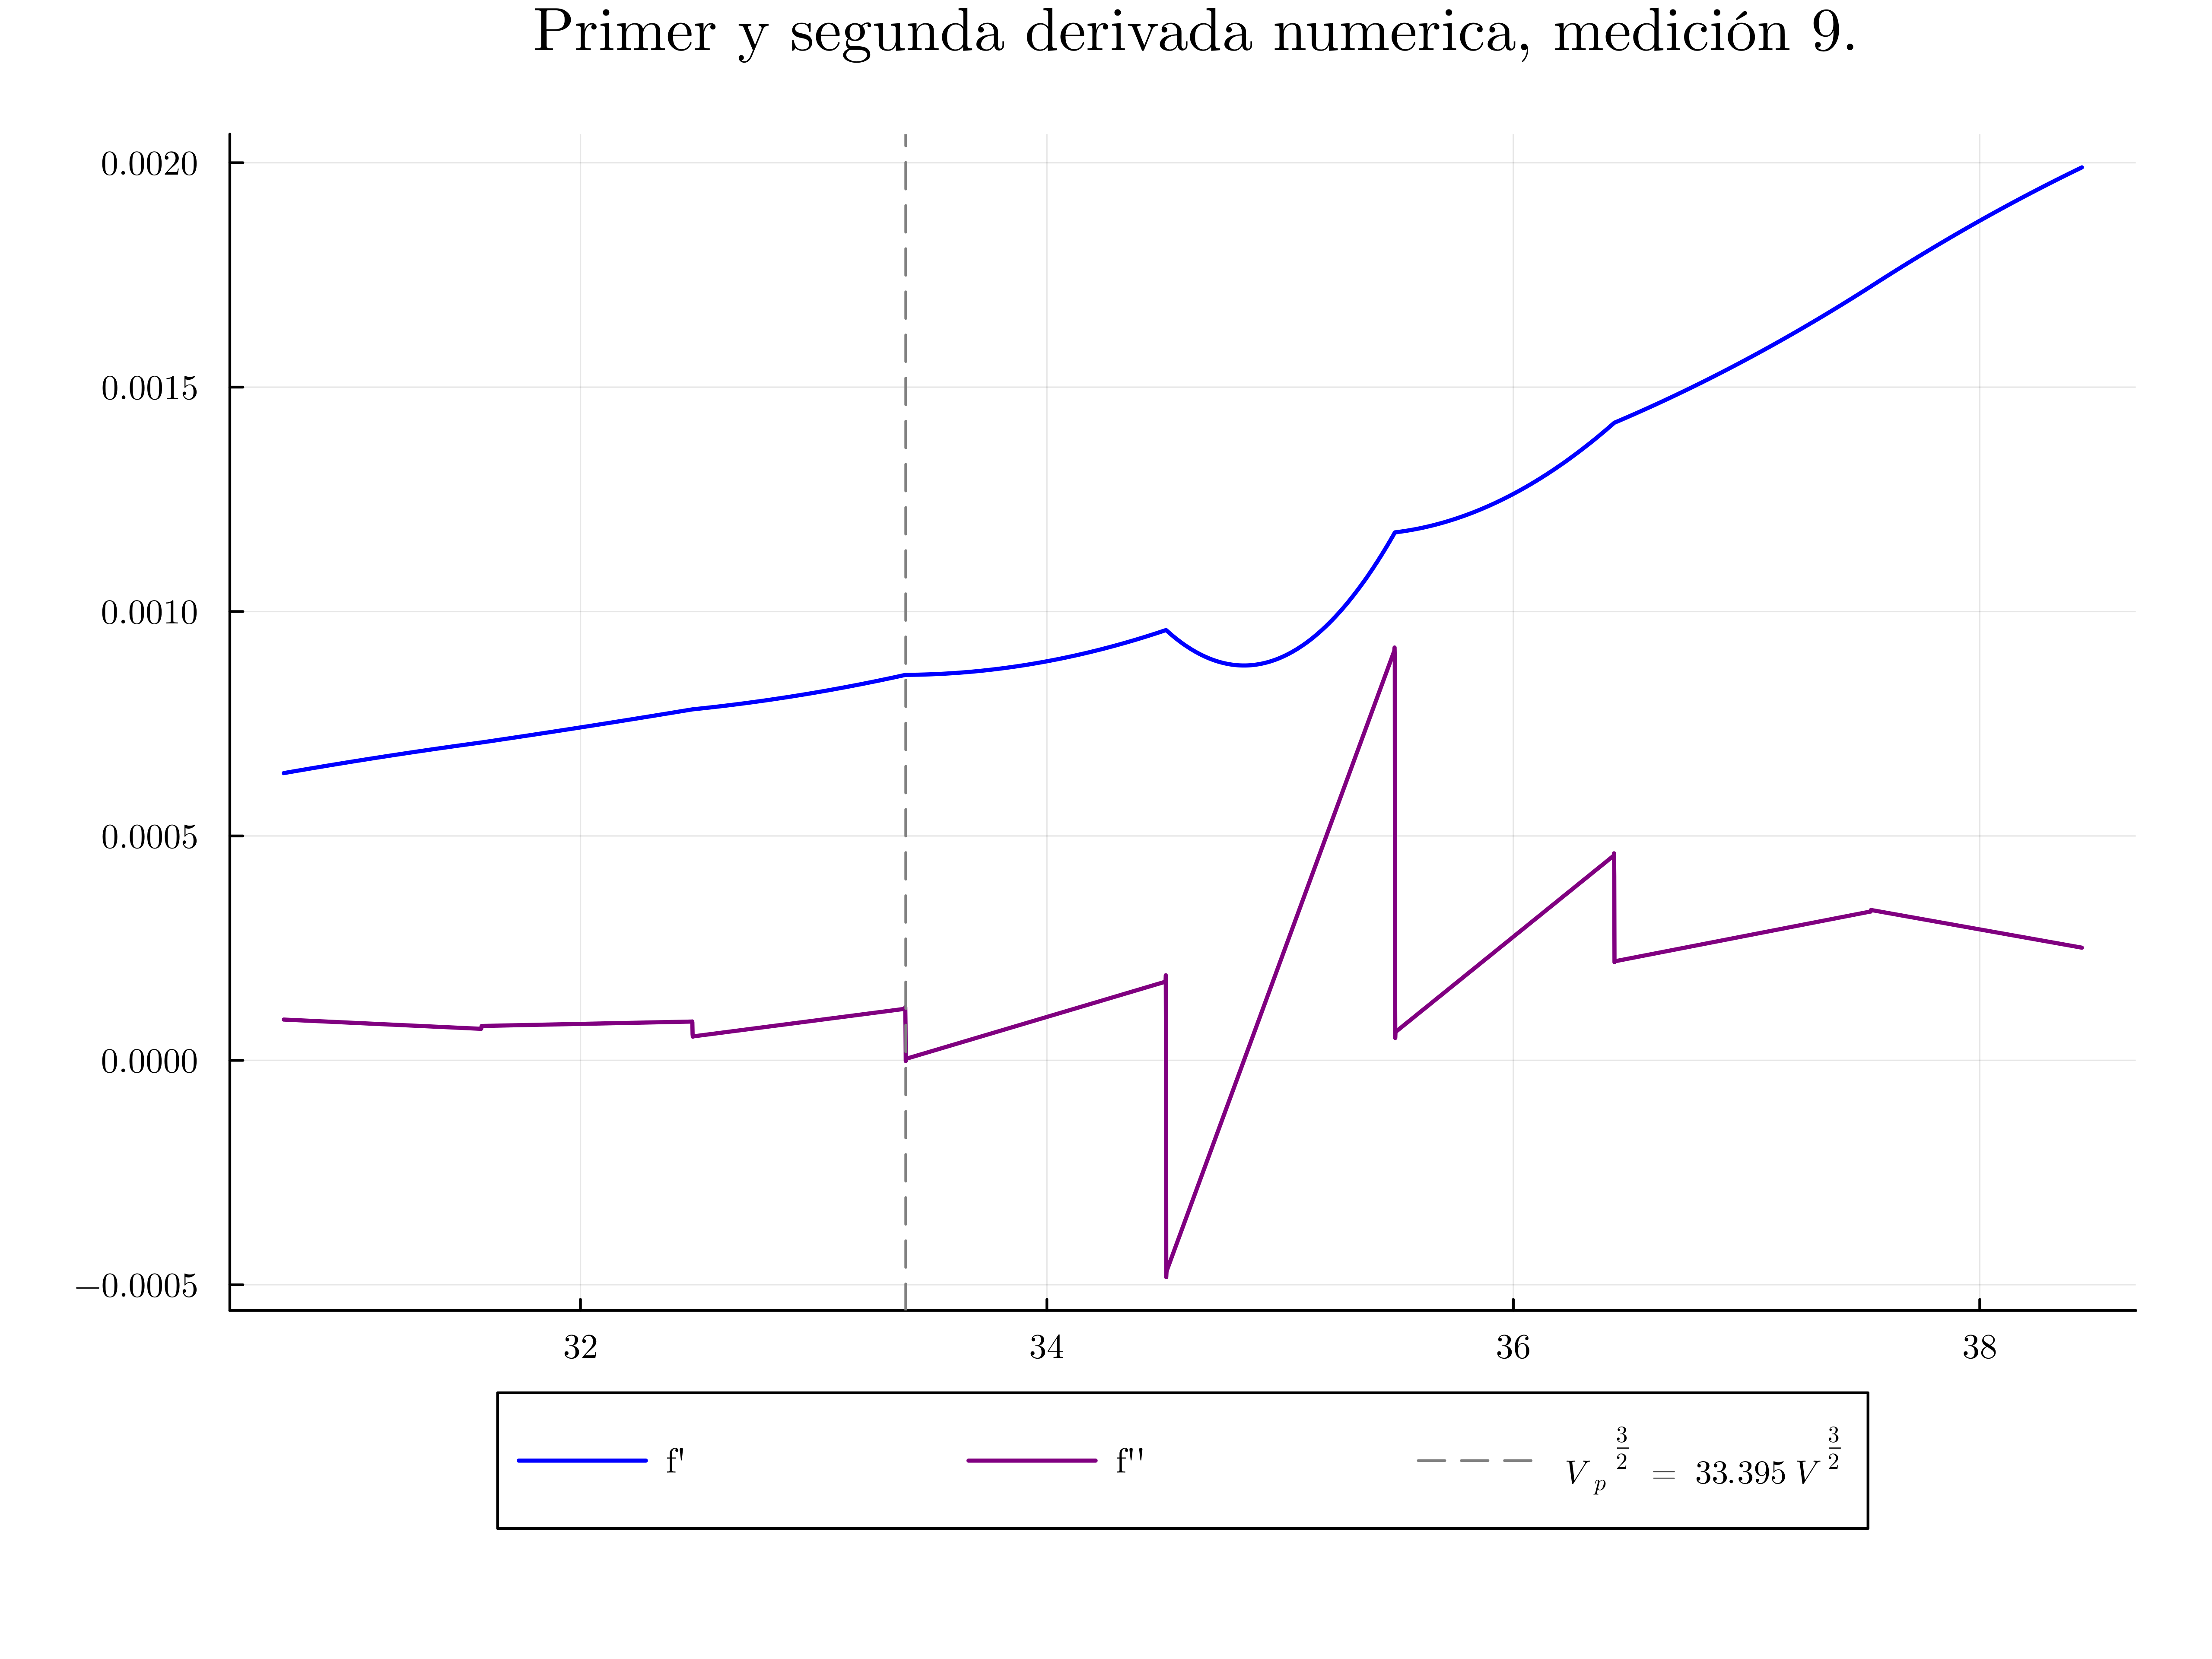
\includegraphics[width=\linewidth]{img/potderps9.png}
	\caption{Barrido n°: 9}
	\label{fig:potderps9}
\end{subfigure}
\hfill
\begin{subfigure}[b]{0.49\textwidth}
	\centering
	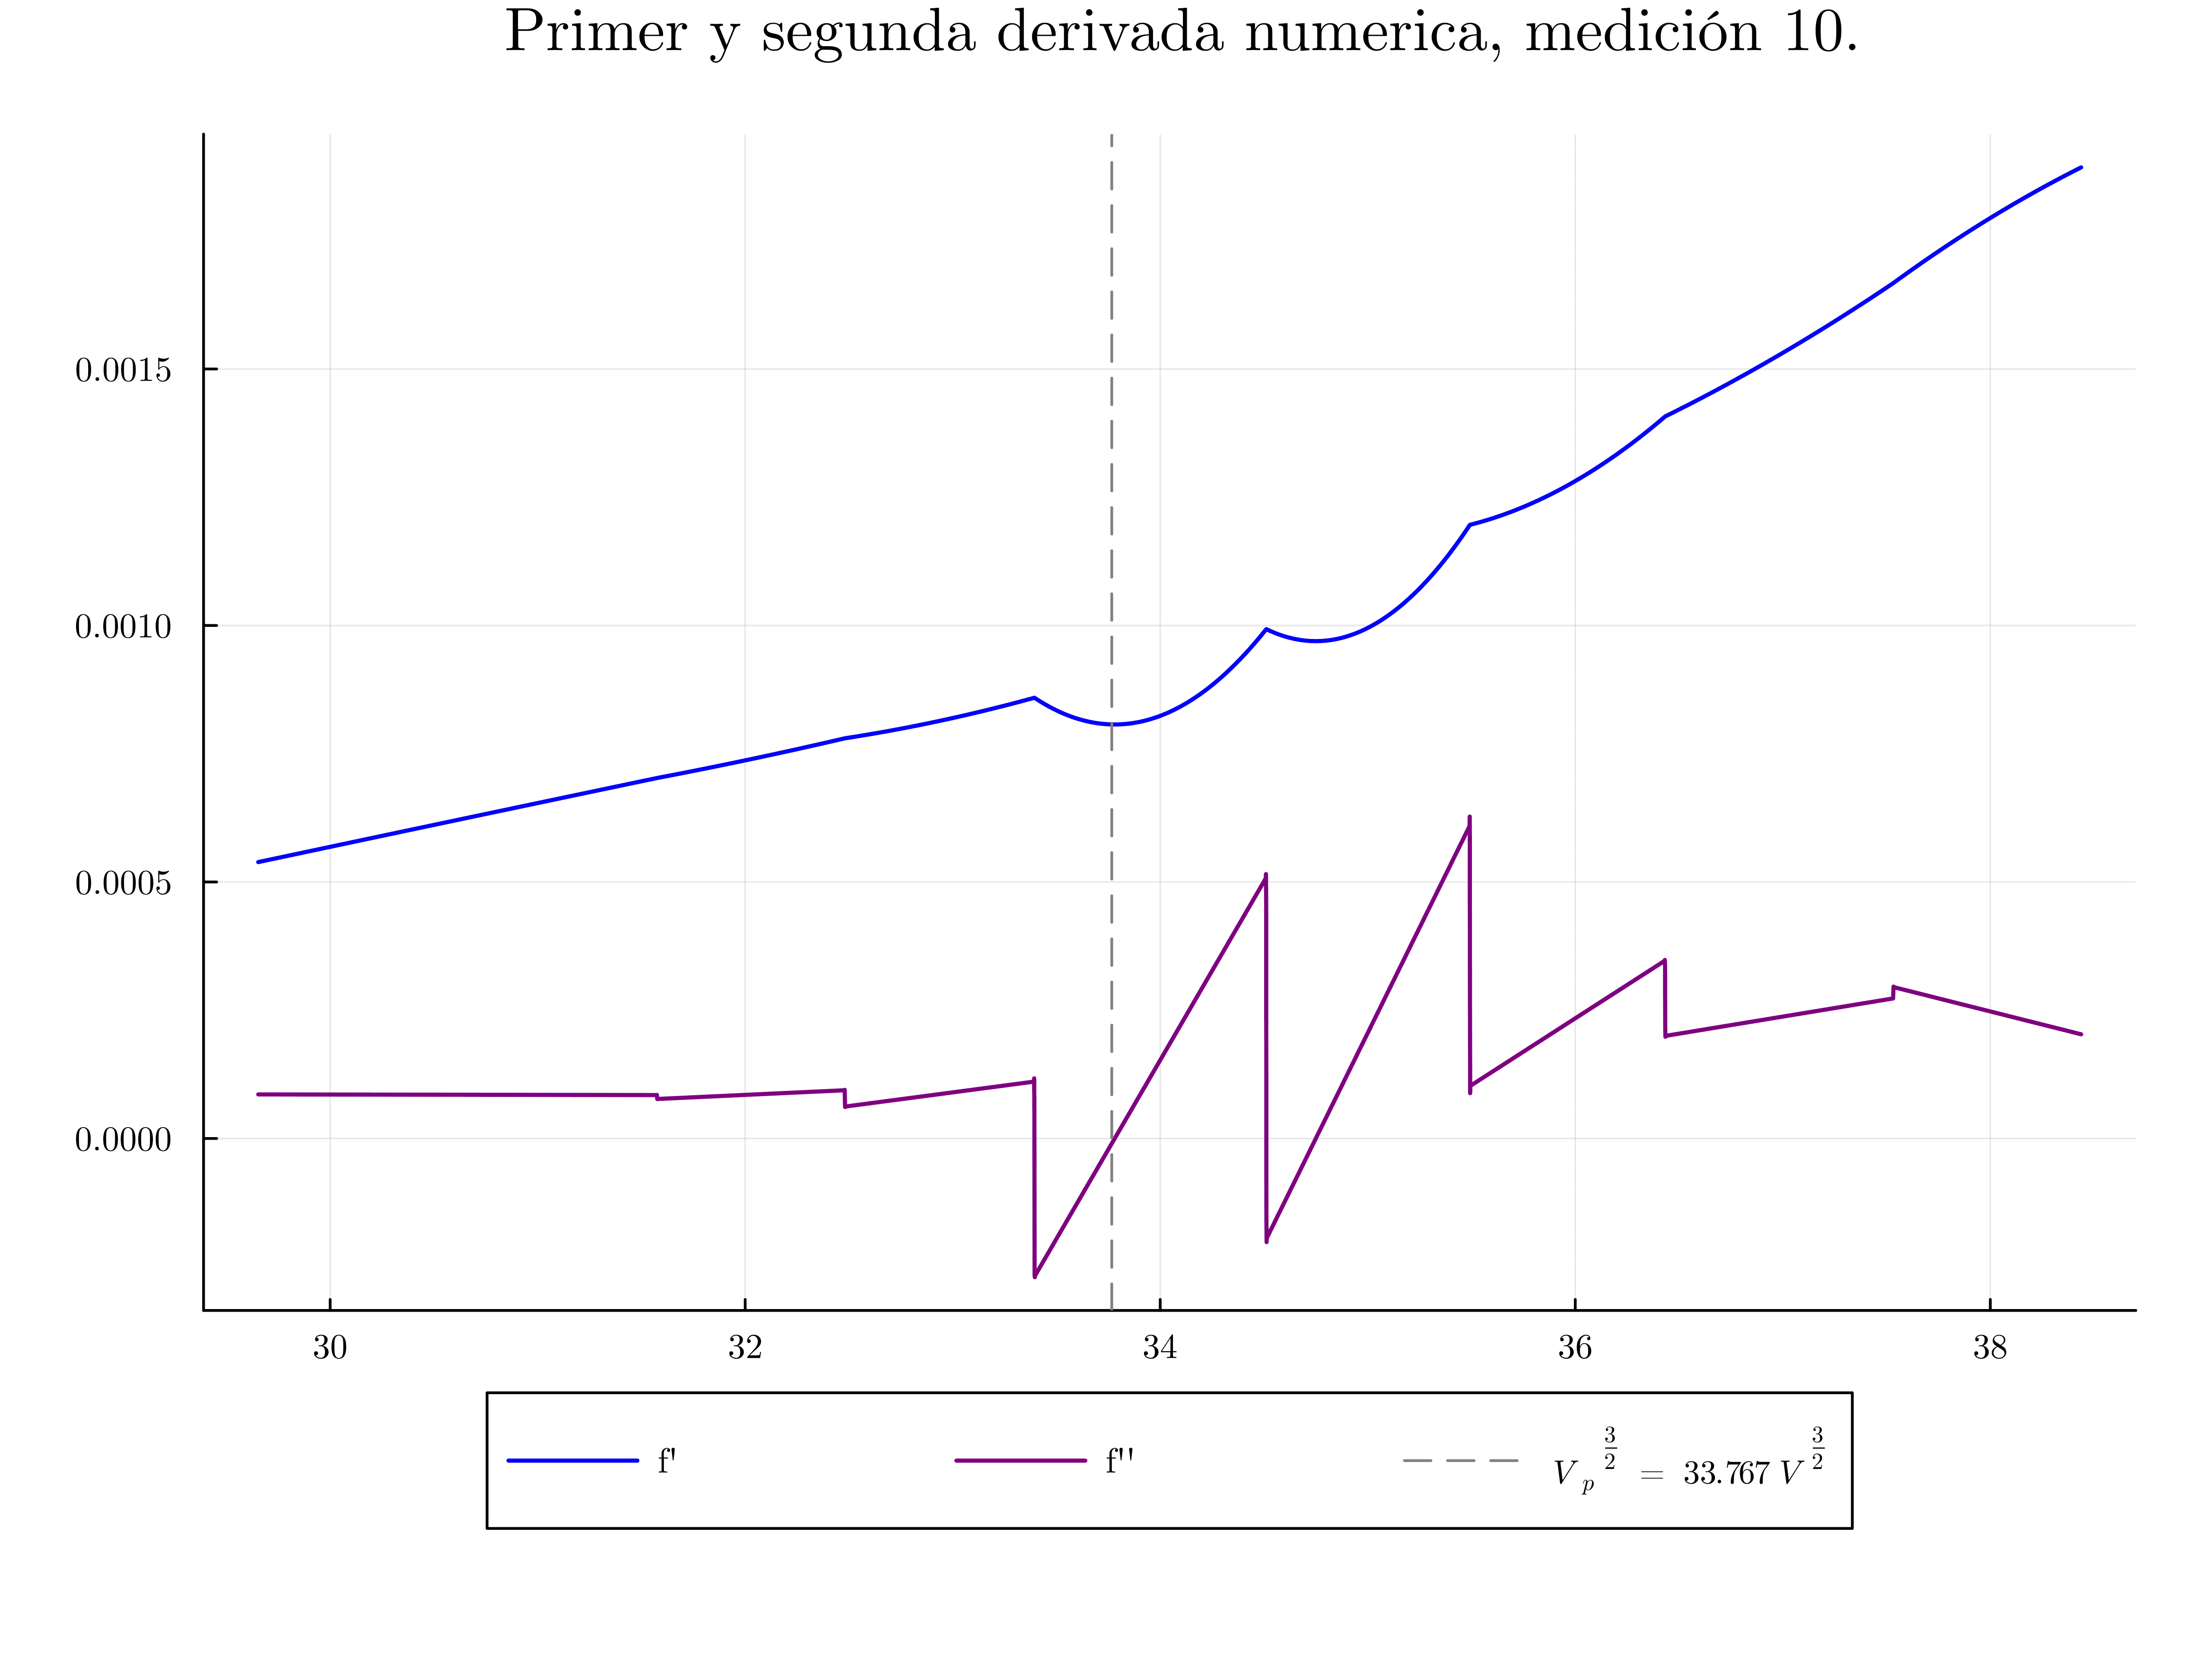
\includegraphics[width=\linewidth]{img/potderps10.png}
	\caption{Barrido n°: 10}
	\label{fig:potderps10}
\end{subfigure}

\caption{Primer y segunda derivada de la corriente del andado con respecto a $V^{\nicefrac{3}{2}}$, para los 10 barridos realizados, donde se puede apreciar la presencia en general de cuatro puntos donde la segunda derivada numérica se acerca a cero, además se puede apreciar que la primera derivada numérica no es suave. Estos fenómenos son causados debido al ruido de la corriente medida el cual se ve trasladado en el algoritmo de LOESS al cambiar en este región múltiples veces de curvatura para ajustar una curva suave, por lo que el punto de inflexión no puede ser detectado de forma gráfica y debe ser determinado mediante el punto en el dominio de $f^{\prime \prime}$ cuyo error con respecto al cero sea menor a $1\times10^{-5}$.}
\label{fig:potderps}
\end{figure}

\twocolumngrid

\bibliographystyle{ieeetr}
\bibliography{citas}

\end{document}
